%!TEX output_directory = texaux
%!TEX spellcheck

\documentclass[polish,mgr,shortabstract]{iithesis}

\usepackage[utf8]{inputenc}

\polishtitle{Sieci neuronowe w systemach dialogowych}
\englishtitle{Neural Networks in Dialogue Systems}
\polishabstract{%!TEX output_directory = texaux
%!TEX spellcheck
%!TEX root = ../main.tex

Praca stanowi przedstawienie niektórych mechanizmów neuronowych wykorzystywanych przy tworzeniu systemów dialogowych, czyli programów komputerowych potrafiących prowadzić rozmowę z użytkownikiem. Pokazuję również jak opisywane metody sprawdzają się w praktyce.

Zaimplementowałem i przetestowałem algorytmy do statystycznego modelowania oraz generowania dialogu. Eksperymentowałem także z architekturą odpowiadającą na pytania o fakty zadawane w języku naturalnym. Do tej ostatniej części dołączam moją próbę rozszerzenia możliwości algorytmu.

}
\englishabstract{%!TEX output_directory = texaux
%!TEX spellcheck
%!TEX root = ../main.tex

\noindent
In this thesis I present selected neural mechanisms used in creating dialogue systems, or computer programs designed to hold a conversation with a user. I also show how methods described here perform in practice.

I implemented and tested algorithms for statistical modeling of a dialogue, as well as dialogue generation. In addition, I experimented with an architecture able to answer questions formulated in natural language. This part also contains my attempt of expanding the capabilities of the system.}
\author{Maciej Pawlikowski}
\advisor{dr Jan Chorowski}
\date{\today}

\usepackage[T1]{fontenc}
\usepackage{lmodern}
\usepackage{amsfonts}            % mathbb
\usepackage{esvect}              % strzałka nad wektorem
\usepackage{amsmath}             % blok aligned
\usepackage{soulutf8}            % łamane podkreślenie
\usepackage{graphicx}            % obrazki
\usepackage{float}               % położenie obrazków w tekście
\usepackage[ruled]{algorithm2e}  % algorytmy
\usepackage{breakcites}          % łamanie cytatów
\usepackage{enumitem}            % wcięcie przy itemize
\usepackage{makecell}            % łamanie wierszy w komórkach
\usepackage{caption}             % odstęp między tabelką a podpisem
\usepackage{gensymb}             % stopień (symbol)
\usepackage{hhline}              % krawędzie tabeli kompatybilne z kolorami


\DeclareMathOperator{\argmax}{arg\,max}

\begin{document}

\captionsetup[table]{skip=8pt}
\renewcommand{\tablename}{Tabela}

%!TEX output_directory = texaux
%!TEX spellcheck
%!TEX root = ../main.tex

\setlength{\abovedisplayskip}{20pt}
\setlength{\belowdisplayskip}{20pt}

\chapter{Wstęp}

System dialogowy (inaczej \textit{chatbot}) to program komputerowy umożliwiający porozumienie w języku naturalnym między człowiekiem a maszyną. Możliwość naturalnej rozmowy z komputerem była kiedyś utożsamiana ze sztuczną inteligencją. Alan Turing, w swojej słynnej publikacji \cite{turing}, pytał czy da się napisać program konwersacyjny, którego ludzki obserwator nie byłby w stanie odróżnić od człowieka. Eksperyment ten dzisiaj nosi miano testu Turinga. Jego obecną formą jest Nagroda Loebnera -- coroczny konkurs, w którym twórcy programów starają się oszukać sędziów. Dotychczas wręczano jedynie nagrodę dla najlepszego chatbota. Nagrody głównej, jednorazowo przyznawanej programowi nieodróżnialnemu od człowieka, nie zdobył jeszcze żaden bot.

Przejście testu Turinga nie jest jednak celem każdego systemu dialogowego. Dzisiejsze chatboty mogą mieć bardzo różne przeznaczenie. Obecna w systemie iOS Siri\footnote{\url{https://www.apple.com/ios/siri/}} stanowi interaktywną pomoc dla użytkownika. Zastosowanie wykrywania mowy umożliwia wydawanie urządzeniu poleceń głosowych w języku naturalnym. Robot będący częścią portalu Visit Wroclaw\footnote{\url{https://www.facebook.com/visitwro/}} pełni rolę informacji turystycznej. Bardzo popularny Cleverbot\footnote{\url{http://www.cleverbot.com/}} cały czas uczy się lepiej mówić wykorzystując historię przeprowadzanych dialogów. Jest to system ogólnego przeznaczenia, potrafiący rozmawiać na wiele tematów. W biznesie chatboty często pełnią rolę interaktywnych asystentów, pomagając znaleźć połączenia lotnicze, zarezerwować miejsca w restauracji, czy zapoznać się z ofertą firmy.

Techniczne aspekty konstrukcji chatbotów również mogą się drastycznie różnić. Napisany w 1995 roku system \textit{Artificial Linguistic Internet Computer Entity} (w~skrócie A.L.I.C.E. lub Alice) \cite{alice} formułuje odpowiedzi wykorzystując dopasowanie wzorca i wypełnianie luk w schematach. Alice wymaga dużej liczby ręcznie utworzonych reguł, co ją mocno ogranicza. Obecnie często eksperymentuje się z wykorzystaniem metod uczenia maszynowego do budowania botów dialogowych. Szczególnie popularne są sieci neuronowe, które w ostatnich latach znacznie zwiększyły nasze możliwości w dziedzinie przetwarzania języka naturalnego.

\section{Cel i zawartość pracy} \label{celpracy}

Celem tej pracy jest przedstawienie niektórych mechanizmów neuronowych znajdujących zastosowanie w systemach konwersacyjnych. Rozdział~\ref{rozdzial1} stanowi wstęp do tematu sieci neuronowych i wprowadzenie niezbędnej nomenklatury. Kolejny opisuje statystyczne modelowanie języka, które jest podstawą sieci pracujących na języku naturalnym. Następne dwa rozdziały są główną częścią pracy. Rozdział~\ref{rozdzial3} pokazuje architekturę generującą wypowiedzi w dialogu korzystając z pojedynczych słów. Zamieszczam tam także przykłady otrzymanych dialogów. Rozdział~\ref{rozdzial4} jest opisem modelu potrafiącego wyciągać z tekstu odpowiedzi na pytania. Zawiera on też moją próbę rozszerzenia oryginalnej funkcji algorytmu, wraz z wynikami. Do pracy dołączone są implementacje opisywanych metod w Pythonie oraz instrukcja powtórzenia eksperymentów. Ze względu na uniwersalność i dostępność danych w przykładach korzystam z języka angielskiego.

Podczas przygotowywania tego opracowania byłem członkiem reprezentacji Uniwersytetu Wrocławskiego na NIPS 2017 Conversational Intelligence Challenge\footnote{\url{http://convai.io/}}. Celem konkursu było zaprogramowanie chatbota rozmawiającego o zadanym na początku rozmowy krótkim artykule. Zaprezentowany przez UWr robot \texttt{poetwanna.be} zdobył w zawodach 1. miejsce ex aequo. Mój wkład obejmował między innymi obsługę trudniejszych pytań o fakty. Udział w konkursie był przyczyną powstania rozdziału~\ref{rozdzial4} tego opracowania, oraz motywacją do przeprowadzenia opisanego w~sekcji~\ref{negans} eksperymentu z negatywnymi odpowiedziami.

%!TEX output_directory = texaux
%!TEX spellcheck
%!TEX root = ../main.tex

\setlength{\abovedisplayskip}{20pt}
\setlength{\belowdisplayskip}{20pt}

\chapter{Sieci neuronowe} \label{rozdzial1}

\section{Wprowadzenie}
Sieci neuronowe to popularna w ostatnich czasach metoda uczenia maszynowego. Nazwa może słusznie przywodzi na myśl połączenia w mózgu, ponieważ właśnie one były inspiracją stojącą za powstaniem opisywanych algorytmów. Czasami używa się nazwy \textit{sztuczne sieci neuronowe}, dla wyraźnego odróżnienia ich od biologicznych odpowiedników.

Sztuczne sieci neuronowe można krótko opisać jako bardzo złożone, różniczkowalne funkcje, których parametry optymalizowane są za pomocą metod gradientowych. Żeby zastosować sieć neuronową w danym problemie, musimy spełnić dwa warunki:
\begin{itemize}
\item zdefiniować różniczkowalną funkcję kosztu;
\item zgromadzić odpowiednią ilość danych uczących, na których będziemy tę funkcję obliczać i minimalizować.
\end{itemize}

W niektórych zadaniach te wymogi mogą okazać się trudne do spełnienia. Jest to cena, którą ponosimy za uniwersalność tej metody. Ta uniwersalność sprawia, że sieci neuronowe mają zastosowanie w szerokiej gamie problemów uczenia maszynowego, od klasyfikacji \cite{imagenet}, przez kompresję obrazu \cite{compression}, aż do przetwarzania języka naturalnego \cite{rnnlm}.

Żeby ułatwić opisywanie budowy sieci neuronowej, dzieli się ją na mniejsze fragmenty nazywane warstwami. Umożliwia to składanie skomplikowanych architektur z uniwersalnych modułów. Każda warstwa sama w sobie również jest małą siecią. Możemy w uproszczeniu opisać sieć neuronową jako złożenie pewnej liczby warstw. Wektor wejściowy $x \in \mathbb{R}^n$ jest przekształcany w następujący sposób:
\[f(x) = l_L(l_{L-1}(\dots l_1(x \mid \theta_1) \dots \mid \theta_{L-1}) \mid \theta_L),\]
gdzie $L$ jest liczbą warstw, a $l_i$, parametryzowana przez zbiór $\theta_i$, funkcją obliczaną przez $i$-tą warstwę. Musi ona być różniczkowalna względem swoich parametrów. Funkcja $f$ stanowi koszt, który chcemy zminimalizować i jest zależna od $\theta = \bigcup_{i=1}^L \theta_i$.

\noindent
Wizualnie taką sieć reprezentuje ścieżka:

\begin{figure}[H]
  \centering
    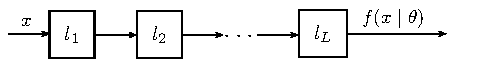
\includegraphics[width=0.8\textwidth]{chapter1/img/prosta.eps}
  \caption{\small{Schemat sieci neuronowej o strukturze liniowej.}}
\end{figure}

\noindent
Jest to pewne uproszczenie, bo nic nie stoi na przeszkodzie, żeby sieć wyglądała tak:

\begin{figure}[H]
  \centering
    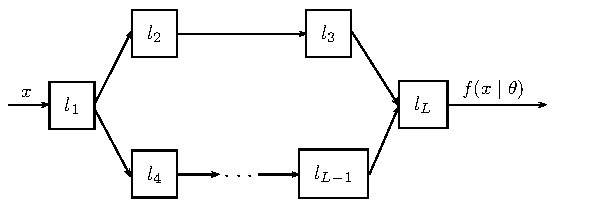
\includegraphics[width=0.9\textwidth]{chapter1/img/dag.eps}
  \caption{\small{Schemat przykładowej sieci neuronowej o strukturze DAG.}}
\end{figure}

W drugim przypadku funkcją wyliczaną przez $l_L$ może być na przykład długość konkatenacji obu wejść, albo suma elementów wyniku $l_{L-1}$ o pozycjach zadanych wynikiem $l_3$. Topologia sieci neuronowej ściśle zależy od zastosowania.

%%%%%%%%%%%%%%%%%%%%%%%%%%%%%%%%%%%%%%%%%%%%%%%%%%%%%%%%%%%%%%%%%%%%%%%%%

\section{Uczenie sieci neuronowej}
Dla uproszczenia przedstawię proces optymalizacji sieci przedstawionej na rysunku 1. Przypomnijmy, że dla punktu danych $x \in \mathbb{R}^n$ funkcja kosztu jest zadana wzorem
\[f(x) = l_L(l_{L-1}(\dots l_1(x \mid \theta_1) \dots \mid \theta_{L-1}) \mid \theta_L),\]
gdzie dla każdego $i$ $l_i$ jest funkcją parametryzowaną przez $\theta_i$, posiadającą pochodne cząstkowe względem elementów $\theta_i$. Funkcja $f$ jest zatem różniczkowalna względem elementów $\theta$. Załóżmy dodatkowo, że zbiory $\theta_1, \dots, \theta_L$ są parami rozłączne.

%%%%%%%%%%%%%%%%%%%

\subsection{Propagacja wsteczna}
Do optymalizacji $\theta$ wykorzystujemy metody gradientowe. Interesuje nas zatem obliczenie pochodnych cząstkowych $f$ względem jej parametrów.
\\\\
Wprowadźmy pomocnicze oznaczenie. Niech
\[o_i(x) = l_i(l_{i-1}(\dots l_1(x \mid \theta_1) \dots \mid \theta_{i-1}) \mid \theta_i).\]
Możemy teraz napisać
\[o_i(x) = l_i(o_{i-1}(x) \mid \theta_i)\]
oraz
\[f(x) = o_L(x).\]
\\
Przydatny będzie też fakt, że $o_i$ zależy tylko od $x$ oraz $\bigcup_{j=1}^i \theta_j$.
\\

Pochodne obliczamy korzystając z reguły łańcuchowej. Weźmy $t_L \in \theta_L$. Dla czytelności zapisu pominę argumenty funkcji. Dostajemy
\[\frac{\partial f}{\partial t_L} = \frac{\partial o_L}{\partial t_L} = \frac{\partial l_L}{\partial t_L}(o_{L-1}).\]

Ponieważ $o_{L-1}$ nie zależy od $t_L$, tutaj obliczenia się kończą. Dla przykładu weźmy teraz $t_{L-3} \in \theta_{L-3}$. Mamy
\[
\begin{aligned}
    \frac{\partial f}{\partial t_{L-3}} &= \frac{\partial o_L}{\partial t_{L-3}} = \frac{\partial l_L}{\partial o_{L-1}} \frac{\partial o_{L-1}}{\partial t_{L-3}} = \frac{\partial l_L}{\partial o_{L-1}} \frac{\partial l_{L-1}}{\partial o_{L-2}} \frac{\partial o_{L-2}}{\partial t_{L-3}} = \\[10pt]
    &= \frac{\partial l_L}{\partial o_{L-1}} \frac{\partial l_{L-1}}{\partial o_{L-2}} \frac{\partial l_{L-2}}{\partial o_{L-3}} \frac{\partial o_{L-3}}{\partial t_{L-3}}
    = \frac{\partial l_L}{\partial o_{L-1}} \frac{\partial l_{L-1}}{\partial o_{L-2}} \frac{\partial l_{L-2}}{\partial o_{L-3}} \frac{\partial l_{L-3}}{\partial t_{L-3}}(o_{L-4})
\end{aligned}
\]

W przypadku zależności kilku warstw od tego samego parametru konieczne będzie więcej aplikacji reguły łańcucha. Wzory pochodnych cząstkowych komplikują się również dla modeli o bardziej wymyślnej topologii. Ogólna zasada obliczania gradientu funkcji $f$ pozostaje jednak ta sama. W dziedzinie sieci neuronowych proces ten nosi nazwę wstecznej propagacji błędu (ang. \textit{error backpropagation}).\\

%%%%%%%%%%%%%%%%%%%

\subsection{Zbiór uczący i zbiór testowy} \label{testset}

Dotychczas mówiliśmy o funkcji kosztu zadanej na pojedynczym punkcie danych. To jednak za mało, żeby dobrać właściwe parametry. Zwykle trenowanie sieci neuronowych wymaga dużej liczby przykładów. Musimy więc zdefiniować funkcję celu $f_{tot}$ na całym zbiorze danych.

Oznaczmy zgromadzone dane przez $D$. Agregacji wartości $f$ na poszczególnych elementach $D$ często dokonuje się przez uśrednienie:
\[f_{tot}(D \mid \theta) = \frac{1}{|D|} \sum\limits_{d \in D} f(d \mid \theta)\]

Sama minimalizacja $f_{tot}$ nie wystarczy do osiągnięcia satysfakcjonujących rezultatów. Zadaniem modelu nie jest zapamiętanie danych przetwarzanych podczas uczenia, tylko bycie gotowym do pracy z nowymi przykładami. Nie wzięcie tego pod uwagę prowadzi do nadmiernego dopasowania (ang. \textit{overfitting}); model nie będzie w stanie dostarczyć przydanych wyników dla nienapotkanych wcześniej obserwacji. Jest to ogólny problem, często występujący w uczeniu maszynowym.

Istnieje wiele sposobów walki z nadmiernym dopasowaniem (inaczej \textit{regularyzacji} sieci). Mogą one polegać na przykład na zmianach w architekturze modelu lub umyślnym wprowadzaniu zaburzeń w danych. Podstawową metodą, stosowaną niemal zawsze, jest wykorzystanie zbioru testowego. Zgromadzone dane $D$ dzielimy na rozłączne podzbiory $D_{train}$ i $D_{test}$. Dokonujemy optymalizacji $f_{tot}(D_{train} \mid \theta)$. Zbiór $D_{test}$ nie jest bezpośrednio obserwowany przez model. Używamy go jedynie do sprawdzania efektywności modelu na nowych przykładach.

W sieciach neuronowych popularne jest przerywanie procesu uczenia, gdy wartość $f_{tot}(D_{test} \mid \theta)$ nie poprawia się przez zadaną liczbę $k$ kolejnych iteracji (\textit{early stopping}\label{earlys}). Pomaga to uniknąć nieproduktywnych obliczeń i nadmiernego dopasowania. Czasami, zamiast dzielić $D$ na dwa podzbiory, dokonujemy podziału na $D_{train}$, $D_{test}$ i $D_{val}$. Wówczas $D_{val}$ (tzw. zbiór walidacyjny) przejmuje rolę zbioru testowego, a z $D_{test}$ korzystamy tylko raz, dopiero po zakończeniu uczenia. W ten sposób ostateczny wynik jest obliczany w zupełnie nowym środowisku.

\begin{algorithm}[h]
    \SetAlgorithmName{Algorytm}
    \\\\podziel $D$ na rozłączne zbiory $D_{train}$, $D_{test}$, $D_{val}$\\
    $k$ -- maksymalna liczba iteracji bez poprawy\\[5pt]
    losowo zainicjuj $\theta$\\
    \While{\textnormal{była poprawa} $f_{tot}(D_{val} \mid \theta)$ \textnormal{w ostatnich} $k$ \textnormal{iteracjach}}{
        aktualizuj $\theta$ zgodnie z przyjętym algorytmem optymalizacji, korzystając z $\nabla f_{tot}(D_{train})$
    }
    ostateczny koszt to $f_{tot}(D_{test})$
    \caption{Podstawowy schemat uczenia}
\end{algorithm}

W praktyce często zdarza się, że obliczanie $\nabla f_{tot}(D_{train})$ jest bardzo kosztowne ze względu na wielkość zbioru uczącego. Z tego powodu najczęściej przed każdą iteracją losowo dzieli się $D_{train}$ na porcje (ang. \textit{batches}) stałego rozmiaru. Zamiast dokonywać jednej aktualizacji parametrów na iterację, $\theta$ jest modyfikowana po każdej porcji. Optymalizując parametry metodą gradientową traktujemy wejście $x$ jako stałą. Nadużywając oznaczenia, przez $\nabla f_{tot}$ rozumiem wektor pochodnych cząstkowych względem parametrów (nie zawierający $\partial f_{tot} / \partial x$).

\begin{algorithm}[h]
    \SetAlgorithmName{Algorytm}
    \\\\
    \While{\textnormal{była poprawa} $f_{tot}(D_{val} \mid \theta)$ \textnormal{w ostatnich} $k$ \textnormal{iteracjach}}{
        podziel $D_{train}$ na porcje $D_{train}^{(1)}, \dots , D_{train}^{(B)}$\\
        \For{$i \gets 1$ \KwTo $B$}{
            aktualizuj $\theta$ zgodnie z przyjętym algorytmem optymalizacji, korzystając z $\nabla f_{tot}(D_{train}^{(i)})$
        }
    }
    \caption{Wsadowa aktualizacja parametrów}
\end{algorithm}

%%%%%%%%%%%%%%%%%%%

\subsection{Metoda gradientu prostego}
Do minimalizacji funkcji celu względem parametrów sieci zwykle używa się jakiegoś wariantu metody gradientu prostego (ang. \textit{gradient descent}). Jest to iteracyjna metoda optymalizacji. Od punktu startowego poruszamy się w kierunku odwrotnym do gradientu. Dla wypukłej, różniczkowalnej funkcji $g(\theta)$, której pochodna spełnia warunek Lipschitza, następujący algorytm gwarantuje zbieżność do globalnego minimum:
\\[.5cm]
\begin{algorithm}[H]
    \SetAlgorithmName{Algorytm}
    \\\\zaczynamy od pewnego $\theta_0$\\
    $\alpha$ -- tempo uczenia\\[5pt]
    \For{$t \gets 1\ \KwTo\ \infty$}{
        $\theta_t \gets \theta_{t-1} - \alpha \nabla g(\theta_{t-1})$
    }
    \caption{Metoda gradientu prostego}
\end{algorithm}

\vspace{.5cm}

Zbieżność wymaga odpowiedniego doboru tempa uczenia, oraz, być może, jego modyfikacji w kolejnych iteracjach. Oprócz tego w przypadku funkcji obliczanej przez sieć neuronową teoretyczne warunki mogą nie być spełnione, a nawet najczęściej nie są. Sprawia to, że nie ma gwarancji zbieżności opisywanych metod do optymalnego rozwiązania. W praktyce jednak modyfikacje metody gradientu prostego pozwalają z powodzeniem uczyć bardzo skomplikowane sieci. Ponieważ podczas optymalizacji prawdziwej sieci aktualizacji $\theta$ dokonujemy porcjami, pełna nazwa algorytmu to \textit{stochastic gradient descent}, w skrócie \textit{SGD}.

\subsection{\textit{Adaptive Moment Estimation}} \label{adam}
Analiza wariantów \textit{SGD} nie jest tematem tej pracy, więc krótko przedstawię tylko tę wersję, z której korzystałem ucząc moje implementacje. \textit{ADAM} (\textit{adaptive moment estimation}) \cite{adam} wprowadza ważne usprawnienie do podstawowej formuły.

Pojawiają się osobne tempa uczenia dla poszczególnych elementów $\theta$. Parametr, który, ze względu na naturę danych uczących, jest wykorzystywany (a więc i aktualizowany) rzadko, teraz będzie podlegał silniejszym modyfikacjom. Z kolei taki, który pojawia się niemal wszędzie (i jest aktualizowany w prawie każdym kroku), będzie zmieniany bardzo ostrożnie. Pozwala to na większą dokładność w drugim przypadku oraz krótszy proces uczenia w pierwszym. Sprawia także, że ręczny wybór właściwego $\alpha$ przestaje być kluczowy. O tempie zmian parametru w metodzie \textit{ADAM} decydują wartości jego pierwszego i drugiego momentu, których szacowania są aktualizowane w każdym kroku.

\begin{algorithm}[h]
    \SetAlgorithmName{Algorytm}
    \\\\zaczynamy od pewnego $\theta_0$\\
    $\alpha$ -- tempo uczenia\\
    $\beta_1, \beta_2 \in [0,1)$ -- parametry aktualizacji przybliżeń momentów\\[5pt]
    $m_0 \gets 0$ -- wektor pierwszych momentów\\
    $v_0 \gets 0$ -- wektor drugich momentów\\
    \For{$t \gets 1\ \KwTo\ \infty$}{
        $g_t \gets \nabla g(\theta_{t-1})$\\
        $m_t \gets \beta_1 m_{t-1} + (1 - \beta_1) g_t$\\
        $v_t \gets \beta_2 v_{t-1} + (1 - \beta_2) g_t^2$\\
        $\hat{m}_t \gets m_t\ /\, (1 - \beta_1^t)$\\
        $\hat{v}_t \gets v_t\ /\, (1 - \beta_2^t)$\\
        $\theta_t \gets \theta_{t-1} - \alpha \hat{m}_t\ /\, (\sqrt{\hat{v}_t} + \epsilon)$
    }
    \caption{\textit{ADAM}}
\end{algorithm}
\vspace{-10pt}\small\noindent
Wszystkie operacje są nakładane na pojedyncze elementy. Górny indeks oznacza potęgowanie. Autorzy zalecają $\alpha = 10^{-3}$, $\beta_1 = 0.9$, $\beta_2 = 0.999$, $\epsilon = 10^{-8}$.\\[-10pt]
\normalsize

Warto nadmienić, że \textit{ADAM} nie wywodzi się bezpośrednio z \textit{SGD}, lecz stanowi ewolucję pomysłów i ulepszeń wprowadzonych w wielu wcześniejszych metodach, takich jak \textit{momentum} \cite{momentum}, \textit{ADAGRAD} \cite{adagrad}, \textit{ADADELTA} \cite{adadelta}, czy \textit{RMSProp} \cite{rmsprop}.

%%%%%%%%%%%%%%%%%%%%%%%%%%%%%%%%%%%%%%%%%%%%%%%%%%%%%%%%%%%%%%%%%%%%%%%%%

\section{Warstwy}
Warstwy mogą reprezentować bardzo zawiłe przekształcenia. Można jednak wyróżnić kilka najczęściej występujących typów, które stanowią podstawowy budulec większości nowoczesnych sieci. Żeby uniknąć niejasności powtórzmy, że każda warstwa sama w sobie również jest siecią neuronową. Z tego powodu często zamiast, na przykład, \textit{warstwa rekurencyjna} można przeczytać \textit{sieć rekurencyjna} w odniesieniu do tego samego obiektu.

%%%%%%%%%%%%%%%%%%%

\subsection{Warstwa afiniczna}
Najprostszą spotykaną warstwą jest warstwa afiniczna (warstwa pełna, warstwa gęsta). Jest to po prostu mnożenie przez macierz połączone z przesunięciem. Najczęściej przekształcenie kończy się nieliniowością, co pozwala na reprezentowanie skomplikowanych funkcji łącząc kilka warstw afinicznych. Przekształcenie jest zatem zadane wzorem
\[\mathit{f}(x) = \gamma(Ax + b),\]
gdzie $A \in \mathbb{R}^{m \times n}$ i $b \in \mathbb{R}^m$ są parametrami warstwy, a $\gamma$ jest nieliniowością. Notacja $\gamma(W)$ oznacza tutaj zaaplikowanie $\gamma$ do każdego elementu $W$. Taki zapis jest często spotykany w literaturze poświęconej sieciom neuronowym.
\\\\
Popularne wybory $\gamma$ to między innymi:
\begin{itemize}
\item $\gamma(z) = \mathrm{ReLU}(z) = \max(0, z)$, tzw. \textit{rectified linear unit};
\item $\gamma(z) = \sigma(z) = \frac{1}{1 + e^{-z}}$, \textit{sigmoid function};
\item $\gamma(z) = \tanh(z) = \frac{e^z - e^{-z}}{e^z + e^{-z}}$.
\end{itemize}

\vspace{5mm}
Warstwa gęsta stanowi rozwinięcie idei \textit{perceptronu} \cite{perceptron}. Perceptron oblicza znak przesuniętej, ważonej sumy elementów wejścia:
\[f(x) = \mathrm{sgn}(x^Ta + b),\]
gdzie $a \in \mathbb{R}^n$, $b \in \mathbb{R}$ są parametrem modelu, a $\mathrm{sgn}$ funkcją znaku. Może być on wykorzystywany do binarnej klasyfikacji liniowo separowalnych punktów. Pierwsza implementacja perceptronu miała miejsce w 1957 roku. Dzisiaj często służy on za przykład najprostszej sieci neuronowej.

%%%%%%%%%%%%%%%%%%%

\subsection{\textit{Softmax}}
Niektóre problemy wymagają pracy z prawdopodobieństwami. Chcąc na przykład zrobić klasyfikator o różniczkowalnym wyjściu, możemy zbudować model, który dla danego $a$ zwraca prawdopodobieństwa należenia $a$ do poszczególnych klas ze zbioru wszystkich klas $\mathbf{K} = \{1,\dots,K\}$. Wynikiem klasyfikacji jest ta klasa, której prawdopodobieństwo jest największe. W takiej sytuacji często korzysta się z funkcji \textit{softmax}, zdefiniowanej dla $z \in \mathbb{R}^{K}$ następująco:
\[(\mathrm{softmax}(z))_i = \frac{e^{z_i}}{\sum_{k \in \mathbf{K}} e^{z_k}}\]

\textit{Softmax} przekształca dowolny wektor długości $K$ w wektor liczb, które są pewnym dyskretnym rozkładem prawdopodobieństwa na wszystkie klasy. Funkcja $\exp$ funkcjonuje tutaj jako wygodna nieliniowość, dzięki której nie musimy się przejmować ujemnymi wartościami w $z$ i zyskujemy większą siłę wyrazu.

\textit{Softmax} zwykle łączy się z przekształceniem afinicznym. Pełna funkcja obliczana przez warstwę to
\[f(x) = \mathrm{softmax}(Ax + b),\]
\\
gdzie $A \in \mathbb{R}^{K \times n}$ i $b \in \mathbb{R}^{K}$ to parametry. Jest to zatem pewien szczególny przypadek wartswy gęstej, z tą różnicą, że nieliniowość nie jest nakładana na każdy element z~osobna. Dodatkowe mnożenie przez macierz pozwala nam zmienić kształt danych; wejście do funkcji \textit{softmax} musi mieć długość równą liczbie klas. W literaturze pod pojęciem \textit{softmax} może kryć się zarówno cała warstwa, jak i sama funkcja \textit{softmax}.

%%%%%%%%%%%%%%%%%%%

\subsection{Próbkowany \textit{softmax}} \label{ssoft}
\textit{Softmax}, w swojej podstawowej formie, jest mało wydajny w przypadku dużej liczby możliwych etykiet. W pracy z językiem naturalnym rolę etykiet pełnią słowa, a~tych potrafią być setki tysięcy, więc jest to dość częste zjawisko. Podczas uczenia sieci chcemy maksymalizować prawdopodobieństwo właściwej klasy $k_a \in \mathbf{K}$ dla każdego elementu $a$ w zbiorze uczącym. W przypadku klasycznego \textit{softmaxa} mamy
\[\hat{P}(k \mid a) = (\mathrm{softmax}(z))_{k} = \frac{e^{z_{k}}}{\sum_{i \in \mathbf{K}} e^{z_i}},\]
gdzie $z$ zależy od $a$. Zauważmy, że powyższe równanie można zapisać jako
\[z_k = \log(\hat{P}(k \mid a)) + C_0(a)\]
dla pewnej funkcji $C_0$ niezależnej od $k$. Oznacza to, że warstwa w sieci obliczająca $z$ tak naprawdę oblicza przesunięte logarytmy prawdopodobieństw. Oczywiście wartość przesunięcia jest nieistotna dzięki funkcji \textit{softmax}.

Do poznania wartości $\hat{P}(k_a \mid a)$ wystarczy nam tylko jeden element wynikowego wektora. Niestety, nawet do obliczenia jednego elementu musimy znać wartość $\sum_{i \in \mathbf{K}} e^{z_i}$. Przeszkodę stanowi fakt, że zwykle \textit{softmax} łączy się z warstwą afiniczną. Żeby na podstawie wektora wejściowego $x \in \mathbb{R}^n$ obliczyć mianownik \textit{softmaxa}, trzeba nałożyć na $x$ macierz $A \in \mathbb{R}^{K \times n}$, co jest dość kosztowne. Sprawia to, że w przypadku bardzo dużego $K$ zamiast pełnej funkcji \textit{softmax} stosuje się różne przybliżenia. Jednym z nich jest wersja z próbkowaniem (ang. \textit{sampled softmax}) \cite{ssoftmax}.

Opiera się ona na ograniczeniu liczby modyfikowanych parametrów w poszczególnych krokach. Będziemy rozkładać masę prawdopodobieństwa nie na całym $\mathbf{K}$, ale na jakimś mniejszym zbiorze. Pozwoli to nie wykonywać pełnego mnożenia przez macierz $A$, co z kolei spowoduje, że tylko niektóre jej wiersze będą wymagały aktualizacji.

Zaczynamy od wybrania pewnego $Q$ -- rozkładu prawdopodobieństwa na $\mathbf{K}$. Dla każdego $a$ wybieramy stałego rozmiaru próbkę $M_a$, gdzie prawdopodobieństwo wyboru $k$ wynosi $Q(k)$. Losujemy ze zwracaniem, więc $M_a$ może zawierać duplikaty. Do zgromadzonych etykiet dodawana jest właściwa, $k_a$. Nieco nadużywając notacji:
\[\hat{M}_a = M_a \cup \{k_a\}\]

Następnie należy jeszcze raz określić rozkład na $\mathbf{K}$, teraz zaopatrując model w~dodatkowy fakt: $k_a \in \hat{M}_a$. Sieć oczywiście nie wie, która klasa jest właściwa, więc jest to dla niej istotna informacja. Wie natomiast w jaki sposób powstaje zbiór $\hat{M}_a$ i może to wykorzystać obliczając koszt. Oznaczmy prawdopodobieństwo klasy $k$ dla elementu $a$ w tych nowych warunkach jako $\hat{P}(k \mid a, \hat{M}_a)$. Stosując wzór Bayesa otrzymujemy
\[\hat{P}(k \mid a, \hat{M}_a) = \frac{\hat{P}(\hat{M}_a \mid k, a)\, \hat{P}(k \mid a)}{\hat{P}(\hat{M}_a \mid a)},\]
gdzie
\[\hat{P}(\hat{M}_a \mid a) = \sum_{y \in \mathbf{K}} \hat{P}(\hat{M}_a \mid y, a)\, \hat{P}(y \mid a)\]
jest niezależne od $k$.

Zauważmy, że $\hat{P}(\hat{M}_a \mid k, a)$ to po prostu prawdopodobieństwo wylosowania zbioru $\hat{M_a} \setminus \{k\}$ ($M_a = \hat{M_a} \setminus \{k\}$ było wylosowanym zbiorem przy założeniu, że $k_a = k$). Niech dla $i \in \mathbf{K}$ $n_i$ oznacza liczbę wystąpień $i$ w $\hat{M_a}$. Wykorzystując funkcję masy rozkładu wielomianowego dostajemy
\[
\begin{aligned}
    \hat{P}(\hat{M}_a \mid k, a) &= |M_a|! \left[ \prod\limits_{i \in \mathbf{K} \setminus \{k\}} \frac{Q(i)^{n_i}}{n_i!} \right] \frac{Q(k)^{n_k-1}}{(n_k-1)!}= \\[3pt]
    & = |M_a|! \left[ \prod\limits_{i \in \mathbf{K}} \frac{Q(i)^{n_i}}{n_i!} \right]  \frac{Q(k)^{n_k-1}}{(n_k-1)!}  \frac{n_k!}{Q(k)^{n_k}} =\\[3pt]
    & = |M_a|! \left[ \prod\limits_{i \in \mathbf{K}} \frac{Q(i)^{n_i}}{n_i!} \right] \frac{n_k}{Q(k)}.
\end{aligned}
\]

\noindent
Mamy zatem
\[
\begin{aligned}
\hat{P}(k \mid a, \hat{M}_a) &= \frac{|M_a|!}{\hat{P}(\hat{M}_a \mid a)} \left[ \prod\limits_{i \in \mathbf{K}} \frac{Q(i)^{n_i}}{n_i!} \right] \frac{n_k \hat{P}(k \mid a)}{Q(k)}, \\[3pt]
\log(\hat{P}(k \mid a, \hat{M}_a)) &= C_1(a) + \log(\hat{P}(k \mid a)) - \log(Q(k)) + \log(n_k)
\end{aligned}
\]
dla pewnej funkcji $C_1$ niezależnej od $k$. Chcemy nauczyć sieć korzystać z nowej informacji, czyli obliczać
\[\hat{P}(k \mid a, \hat{M}_a) = \frac{e^{z'_{k}}}{\sum_{i \in \hat{M}_a} e^{z'_i}}.\]
Pokazaliśmy, że cel ten jest osiągnięty dla
\[
\begin{aligned}
z'_k &= \log(\hat{P}(k \mid a, \hat{M}_a)) + C_2(a) = \\[3pt]
     &= \log(\hat{P}(k \mid a)) - \log(Q(k)) + \log(n_k) + C_1(a) + C_2(a) = \\[3pt]
     &= z_k - \log(Q(k)) + \log(n_k) + C_3(a)
\end{aligned}
\]

Wartość $C_3(a)$ nie zależy od $k$, więc wystarczy do warstwy obliczającej $z_k$ dodać $- \log(Q(k)) + \log(n_k)$. W mojej implementacji z powodów wydajnościowych pomijam składnik $\log(n_k)$. W praktyce nie wydaje się to mieć negatywnego wpływu na wynik. Pozostaje dobór rozkładu $Q$. Korzystałem tutaj z częstości występowania poszczególnych słów w danych, co dało dobre rezultaty.

%%%%%%%%%%%%%%%%%%%

\subsection{Warstwa rekurencyjna} \label{rnn}
Wiele zadań sztucznej inteligencji wymaga przetwarzania sekwencji. Za przykład może posłużyć tłumaczenie maszynowe. Warstwy gęste nie radzą sobie z tym najlepiej: trzeba ograniczyć się do ciągów konkretnej długości lub przetwarzać sekwencję porcjami, poruszając się po niej oknem o stałym rozmiarze. Warstwa rekurencyjna (ang. \textit{recurrent neural network, RNN}) przetwarza elementy wejścia po kolei, aktualizując swój wewnętrzny stan. Przetwarzanie ciągu $x = (x_1, \dots, x_p), \forall_i x_i \in \mathbb{R}^n$ wygląda tak:
\[
\begin{aligned}
    & h_0 = \vv{0} \in \mathbb{R}^m \\
    & h_t = \gamma(W x_t + U h_{t-1} + b) \\
    & f(x) = h_p \in \mathbb{R}^m
\end{aligned}
\]

Wartości $W \in \mathbb{R}^{m \times n}$, $U \in \mathbb{R}^{m \times m}$, $b \in \mathbb{R}^m$ są parametrami warstwy, a $\gamma$ jest nieliniowością. Stanem początkowym $h_0$ zwykle jest wektor zerowy. W niektórych przypadkach interesują nas rezultaty częściowe. Wówczas wynikiem jest ciąg wektorów lub macierz:
\[f(x) = [h_1\ \dotsb\ h_p] \in \mathbb{R}^{m \times p}\]

Uczenie sieci rekurencyjnej polega na rozwinięciu rekurencji, a następnie konsekwentnym aplikowaniu reguły łańcucha przez całą sekwencję. Metodę tę określa się mianem wstecznej propagacji w czasie (ang. \textit{backpropagation through time, BPTT}).

%%%%%%%%%%%%%%%%%%%

\subsection{\textit{Long Short-Term Memory}} \label{lstm}
Zadaniem sieci rekurencyjnej jest modelowanie sekwencji, co czasami wiąże się z~koniecznością zapamiętywania relacji między odległymi elementami. Opisana wyżej klasyczna wersja teoretycznie jest do tego zdolna, ale optymalizacja jej za pomocą propagacji wstecznej jest bardzo trudna. Powodem jest tzw. problem znikającego gradientu (ang. \textit{vanishing gradient problem}). Wielokrotne aplikowanie reguły łańcucha sprawia, że gradient w kolejnych punktach w czasie maleje wykładniczo, często osiągając wartość bliską zeru już po kilku krokach. Powoduje to zanikanie zależności między wyrazami ciągu mocno oddalonymi w czasie \cite{hardrnn}.

\textit{Long Short-Term Memory} \cite{lstm} to zmodyfikowana wersja tradycyjnej sieci rekurencyjnej. \textit{LSTM} nie ma problemu z modelowaniem relacji pomiędzy odległymi elementami sekwencji. Kluczowym elementem tej warstwy są tzw. bramki, które decydują jak wiele informacji przenieść do kolejnego kroku rekurencji w niezmienionej formie. Pomaga to rozwiązać problem zanikających gradientów. \textit{LSTM} posiada również dodatkową pamięć, w której może przechowywać informację o wybranych wydarzeniach z przeszłości. W ten sposób ma do nich bezpośredni dostęp, więc łatwiej jej znaleźć zależności sięgające daleko wstecz.
\\
Klasyczne równania \textit{LSTM} przedstawiają się następująco:
\[
\begin{aligned}
    & c_0 = h_0 = \vv{0} \in \mathbb{R}^m \\
    & f_t = \sigma(W_f x_t + U_f h_{t-1} + b_f) \\
    & i_t = \sigma(W_i x_t + U_i h_{t-1} + b_i) \\
    & o_t = \sigma(W_o x_t + U_o h_{t-1} + b_o) \\
    & c_t = f_t \odot c_{t-1} + i_t \odot \tanh(W_c x_t + U_c h_{t-1} + b_c) \\
    & h_t = o_t \odot \tanh(c_t)
\end{aligned}
\]
\\
gdzie $b_f, b_i, b_o, b_c \in \mathbb{R}^m$, $W_f, W_i, W_o, W_c \in \mathbb{R}^{m \times n}$, $U_f, U_i, U_o, U_c \in \mathbb{R}^{m \times m}$ są parametrami przekształcenia, a $\odot$ oznacza iloczyn Hadamarda. Podobnie jak poprzednio, w zależności od zastosowania, wyjściem może być $h_p \in \mathbb{R}^m$ lub $[h_1 \dotsb h_p] \in \mathbb{R}^{m \times p}$.

Dodatkowa pamięć to wektor $c_t$. Jego aktualizacja przebiega w dwóch etapach. Najpierw następuje decyzja, które wartości pamięci należy przenieść do następnego kroku i w jakim stopniu. Odpowiada za to bramka $f_t$ (\textit{forget gate}). Następnie dodajemy do pamięci informacje o aktualnym elemencie. Bramka $i_t$ (\textit{input gate}) odpowiada za wybranie istotnych fragmentów przetworzonego wejścia. Kolejny stan, $h_t$, powstaje przez przepuszczenie pamięci przez $o_t$ (\textit{output gate}).

Eksperymenty \cite{gatesvstanh} pokazują, że \textit{LSTM} modeluje sekwencje dużo lepiej niż zwykła warstwa rekurencyjna. Dzisiaj jest to dominujący sposób implementacji rekurencji w sieci neuronowej. Wielu autorów używa pojęcia \textit{RNN}, w~rzeczywistości mając na myśli jakiś wariant \textit{LSTM}.

%%%%%%%%%%%%%%%%%%%

\subsection{\textit{Gated Recurrent Unit}}
Popularną alternatywą dla \textit{LSTM} jest zaproponowana niedawno \textit{GRU} (\textit{gated recurrent unit}) \cite{encdec}. Niesie ona ze sobą pewne uproszczenie architektury. Bramki $f_t$ i $i_t$ zostały połączone w jedną \textit{update gate}, $u_t$. Rolę zapominania informacji przejęła nowa bramka $r_t$, \textit{reset gate}. Nie ma dodatkowej pamięci. Zmiany te skutkują mniejszą liczbą parametrów i nieco niższą złożonością obliczeniową. Mimo to efektywność \textit{GRU} jest porównywalna z \textit{LSTM} \cite{gatesvstanh}.
\\
Pełna definicja warstwy:
\[
\begin{aligned}
    & h_0 = \vv{0} \in \mathbb{R}^m \\
    & u_t = \sigma(W_u x_t + U_u h_{t-1} + b_u) \\
    & r_t = \sigma(W_r x_t + U_r h_{t-1} + b_r) \\
    & \tilde{h_t} = \tanh (W x_t + U (h_{t-1} \odot r_t)  + b) \\
    & h_t = (1 - u_t) \odot h_{t-1} + u_t \odot \tilde{h_t}
\end{aligned}
\]
\\
gdzie $b_u, b_r, b \in \mathbb{R}^m$, $W_u, W_r, W \in \mathbb{R}^{m \times n}$, $U_u, U_r, U \in \mathbb{R}^{m \times m}$.

%%%%%%%%%%%%%%%%%%%

\subsection{Dwukierunkowa \textit{RNN}} \label{birnn}
Przejście po sekwencji w jednym kierunku może czasami okazać się niewystarczające. Im dłuższy ciąg, tym więcej informacji o początkowych elementach zostaje zniekształcone lub zapomniane. Czasami najnowsze elementy są najważniejsze, ale zdarza się, że ciąg stanowi zwartą całość, w której wszystkie wyrazy są bardzo istotne. Tak jest w przypadku zdań w języku naturalnym. Żeby lepiej analizować tego typu sekwencje, można skorzystać z dwukierunkowej sieci rekurencyjnej (ang. \textit{bi-directional RNN}, \textit{BRNN} lub \textit{BiRNN}).

W \textit{BiRNN} tak naprawdę mamy do czynienia z dwiema sieciami rekurencyjnymi, o osobnych zestawach parametrów. Pierwsza, $f$, przechodzi po wejściu $x = (x_1, \dots, x_p)$ tak jak zostało to opisane w sekcji~\ref{rnn}, produkując ciąg $(h_1, \dots, h_p)$. Druga, $f_r$, czyta $x$ od końca i zwraca $({h_r}_1, \dots, {h_r}_p)$:
\[
\begin{aligned}
    & f(x) = [h_1 \dotsb h_p] \in \mathbb{R}^{m \times p} \\[8pt]
    & {h_r}_0 = \vv{0} \in \mathbb{R}^{m_r} \\
    & {h_r}_t = \gamma(W_{r} x_{p-t+1} + U_r {h_r}_{t-1} + b_r) \\
    & f_r(x) = [{h_r}_1 \dotsb {h_r}_p] \in \mathbb{R}^{m_r \times p}
\end{aligned}
\]
gdzie $m_r$ jest rozmiarem stanu sieci wstecznej, a $W_r \in \mathbb{R}^{m_r \times n}$, $U_r \in \mathbb{R}^{m_r \times m_r}$, $b_r \in~\mathbb{R}^m_r$ są jej parametrami.

Następnie oba ciągi wyjściowe są agregowane do jednego wyniku. Prostym sposobem na zachowanie wszystkich informacji jest konkatenacja wektorów:
\[f_{bi}(x) =
\begin{bmatrix}
    h_1\\
    {h_r}_1
\end{bmatrix} \in \mathbb{R}^{(m + m_r)}
\]
lub też, w zależności od potrzeb:
\[f_{bi}(x) =
\begin{bmatrix}
    \begin{aligned}
        &h_1 &\dotsb \hspace{.3cm} &h_p\\
        &{h_r}_1 &\dotsb \hspace{.3cm} &{h_r}_p
    \end{aligned}
\end{bmatrix} \in \mathbb{R}^{(m + m_r) \times p}
\]

%!TEX output_directory = texaux
%!TEX spellcheck
%!TEX root = ../main.tex

\setlength{\abovedisplayskip}{20pt}
\setlength{\belowdisplayskip}{20pt}

\chapter{Neuronowy model języka}
Wiele mechanizmów przetwarzania języka naturalnego za pomocą sieci neuronowej opiera się na podobnej podstawie. Jest nią probabilistyczny model języka wykorzystujący sieć rekurencyjną do przetwarzania pojawiających się sekwencji (ang. \textit{recurrent neural network language model, RNNLM}). Model ten jest elementem kluczowym w dalszej części pracy, więc poświęcę ten rozdział na jego opis.

%%%%%%%%%%%%%%%%%%%%%%%%%%%%%%%%%%%%%%%%%%%%%%%%%%%%%%%%%%%%%%%%%%%%%%%%%

\section{Modelowanie występowania słów}
Probabilistyczne modelowanie języka polega na określeniu prawdopodobieństw wystąpienia każdego z możliwych słów w danym kontekście. W przypadku \textit{RNNLM} przyjmujemy, że szansa na wystąpienie danego słowa zależy od całej historii. Kontekstem zatem jest dla nas cała sekwencja poprzedzająca dany wyraz. Prowadzi to do następującej zależności:
\[P(w_1^T) = \prod\limits_{t=1}^T P(w_t \mid w_1^{t-1})\]

Zapis $w_i^j$ oznacza podciąg $(w_i, w_{i+1} \dots, w_j)$, $w_1^T$ to pełen ciąg, a $P(w_1 \mid w_1^{t-1})$ jest prawdopodobieństwem wystąpienia słowa $w_1$ bezpośrednio po sekwencji $w_1^{t-1}$. W przypadku $i > j$, $w_i^j$ jest ciągiem pustym.

%%%%%%%%%%%%%%%%%%%%%%%%%%%%%%%%%%%%%%%%%%%%%%%%%%%%%%%%%%%%%%%%%%%%%%%%%

\section{Architektura sieci}
\textit{RNNLM} składa się z tzw. warstwy zanurzeń, po której następuje warstwa rekurencyjna, a całość kończy się \textit{softmaxem} produkującym prawdopodobieństwa warunkowe, o których była mowa w poprzedniej sekcji. Warstwa zanurzeń (ang. \textit{embedding layer}) odpowiada za przekształcenie sekwencji słów na format liczbowy. Sekcja~\ref{wektory} zawiera więcej informacji na ten temat. Na razie wystarczy, że wejściowa sekwencja słów jest przekształcana na ciąg wektorów, który może być przetwarzany przez sieć rekurencyjną.

Niech $V = \lbrace v_1, v_2, \dots, v_{|V|} \rbrace$ oznacza słownik, czyli zbiór wszystkich słów występujących w języku. Wejściem do sieci jest ciąg $w_1^T$, składający się ze słów. Wygodnie jest o nim myśleć jako o ciągu indeksów, tzn. sekwencja w języku naturalnym to $(v_{w_1}, \dots, v_{w_T})$. Kolejne kroki \textit{RNNLM} wyglądają tak:
\begin{enumerate}
    \item \textbf{Zanurzenia}: ciąg $w_1^T$ jest przetwarzany na $x_1^T$ -- ciąg wektorów w $\mathbb{R}^n$.
    \item \textbf{\textit{RNN}}: sieć rekurencyjna czyta $x_1^T$ produkując $h_1^T$, gdzie $h_i$ jest wynikiem przejścia po $x_1^i$, a $h_0 = \vv{0}$.
    \item \textbf{Softmax}: dla każdego $i \in \{0,\dots,T-1\}$ wektor $h_i$ wchodzi do warstwy \textit{softmax}, która najpierw przekształceniem afinicznym wkłada go w $\mathbb{R}^{|V|}$, a następnie funkcją \textit{softmax} przerabia na wektor prawdopodobieństw $p_{i+1}$. W ten sposób powstaje ciąg $p_1^T$, którego każdy element jest pewnym rozkładem prawdopodobieństwa na $V$.
\end{enumerate}

\begin{figure}[H]
  \centering
    \hspace*{2cm}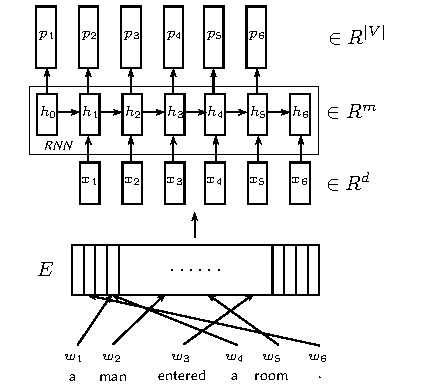
\includegraphics[width=0.9\textwidth]{chapter2/img/rnnlm.eps}
  \caption{\small{Schemat przetwarzania pojedynczej sekwencji przez \textit{RNNLM}. Zamiana słów na wektory odbywa się przez indeksowanie macierzy $E$, $m$ jest rozmiarem stanu \textit{RNN}, a~$d$~rozmiarem zanurzenia.}}
\end{figure}

%%%%%%%%%%%%%%%%%%%%%%%%%%%%%%%%%%%%%%%%%%%%%%%%%%%%%%%%%%%%%%%%%%%%%%%%%

\section{Proces uczenia}
Elementy wynikowego ciągu $p_1^T$ możemy interpretować jako warunkowe rozkłady prawdopodobieństwa na kolejnych pozycjach $w_1^T$. Na przykład $p_3$ określa prawdopodobieństwa poszczególnych słów z $V$ po sekwencji $w_1^2$. Wiemy, że naprawdę pojawiło się tam słowo $w_3$. Według modelu szansa takiego zjawiska to $(p_3)_{w_3}$, czyli element wektora $p_3$ znajdujący się na pozycji $w_3$.

Uczenie neuronowego modelu języka polega na maksymalizowaniu prawdopodobieństw wystąpienia sekwencji, które model faktycznie widzi, czyli tych, co do których zakładamy, że są poprawne. Inaczej mówiąc maksymalizujemy wiarygodność zbioru uczącego. Na podstawie $p_1^T$ możemy obliczyć prawdopodobieństwo zaistnienia całego ciągu. Niech $\theta$ oznacza parametry modelu.
\[\hat{P}(w_1^T\, ;\, \theta) = \prod\limits_{t=1}^T \hat{P}(w_t \mid w_1^{t-1}\, ;\, \theta ) = \prod\limits_{t=1}^T {(p_t)}_{w_t}\]

W praktyce długie iloczyny nie sprawdzają się dobrze ze względu na ograniczenia numeryczne. Chcąc znaleźć parametry maksymalizujące $\hat{P}(w_1^T)$ wystarczy jednak wyznaczyć takie, które maksymalizują $\ln(\hat{P}(w_1^T))$. W uczeniu maszynowym panuje konwencja, według której zwykle minimalizujemy koszt, więc ostateczna forma
optymalizowanej wartości to
\[-\sum\limits_{t=1}^T \ln((p_t)_{w_t}).\]

Jest to bardzo popularna funkcja kosztu, wywodząca się z metody największej wiarygodności. W literaturze nosi nazwę \textit{negative log likelihood}, czasami skracane do \textit{nll}.

%%%%%%%%%%%%%%%%%%%%%%%%%%%%%%%%%%%%%%%%%%%%%%%%%%%%%%%%%%%%%%%%%%%%%%%%%

\section{Reprezentacje wektorowe} \label{wektory}
Większość metod uczenia maszynowego, w tym sieci neuronowe, pracuje na liczbach. Zanim będziemy mogli wprowadzić do algorytmu sekwencje w języku naturalnym, musimy wyznaczyć dla nich odpowiednie liczbowe reprezentacje. Najprostszym pomysłem na przedstawienie słów jako wektorów jest użycie przestrzeni $\mathbb{R}^{|V|}$, w której każde słowo jest kodowane binarnie jako wektor o jednej współrzędnej niezerowej. W ten sposób powstają tzw. rzadkie reprezentacje słów:
\[
\begin{aligned}
    \mathrm{vec_{sparse}}(v_i) &=
    \begin{bmatrix}
        0 \\
        \vdots \\
        0 \\
        1 \\
        0 \\
        \vdots \\
        0
    \end{bmatrix}
\end{aligned} \leftarrow i\text{-ta współrzędna}
\]

Rzadkie wektory mają kilka problemów. Po pierwsze, nie niosą żadnej istotnej informacji o słowach. Jedyna cecha, którą oddają, to kolejność słów w słowniku, co do której i tak nie przyjmujemy żadnych założeń; może być przypadkowa. Po drugie, są bardzo nieefektywne. Używamy tylko jednej współrzędnej, a wymiar może być bardzo duży; słownik może liczyć dziesiątki, a nawet setki tysięcy słów. Ten fakt ma dalsze konsekwencje: macierz $W$ czytającej sekwencje sieci rekurencyjnej musi być bardzo duża.

Rozwiązaniem tych kłopotów jest skorzystanie z gęstych reprezentacji słów, których sieć uczy się jednocześnie z pozostałymi parametrami. Warstwa zanurzeń jest sparametryzowana przez macierz $E \in \mathbb{R}^{d \times |V|}$ o kolumnach $E_1, E_2, \dots, E_{|V|}$, gdzie $d$ jest wybranym rozmiarem zanurzenia. Gęsty wektor dla słowa otrzymujemy mnożąc $E$ przez wektor rzadki, co sprowadza się do wyboru odpowiedniej kolumny:
\[\mathrm{vec_{dense}}(v_i) = E \cdot \mathrm{vec_{sparse}}(v_i) = E_i\]

Podczas minimalizowania kosztu sieć sama będzie szukała optymalnych reprezentacji. Oczekujemy, że dla słów pojawiających się w podobnych kontekstach wyuczone wektory będą podobne. To z kolei powinno spowodować, że prawdopodobieństwa ich wystąpień również okażą się zbliżone.

Okazuje się, że faktycznie tak jest. Otrzymane w ten sposób reprezentacje słów zawierają istotne informacje semantyczne. Podobne słowa dostają bliskie wektory, a~wymiar przestrzeni zanurzeń zostaje znacznie zredukowany (w praktyce najczęściej spotyka się $100 \leq d \leq 300$). Gęste reprezentacje słów okazały się na tyle przydatne, że powstały wyspecjalizowane architektury przeznaczone do ich obliczania. Do najpopularniejszych z nich należą Word2Vec \cite{w2v} i GloVe \cite{glove}.

Jakość otrzymanych wektorów mocno zależy od jakości danych uczących. Małe próbki języka nie dadzą wystarczającej informacji o statystycznym występowaniu słów w kontekstach. Wyuczenie bardzo dobrych zanurzeń słów wymaga zatem dużego zbioru tekstów, a co za tym idzie, pewnego nakładu czasu. Z tego powodu na początkową wartość macierzy $E$ często wybiera się wstępnie obliczone wektory. Skraca to czas potrzebny na znalezienie reprezentacji oraz zmniejsza potrzebną do nauczenia sieci ilość danych. Uczenie zanurzeń zaczynając od takiego ich zainicjowania zwykle pozwala poprawić jakość modelu. Często poprawa jest jednak na tyle mała, że lepiej zaoszczędzić na czasie i potraktować je jako stałe.

Wektory dla języka angielskiego obliczone przez Word2Vec i GloVe są publicznie dostępne. Wykorzystane zbiory danych to odpowiednio korpus Google News, liczący około 100 miliardów słów, i Common Crawl (840 miliardów słów).

Pomysł wykorzystania gęstych wektorów do reprezentowania słów pojawił się po raz pierwszy w \cite{bengiolm}. Tam też został opisany neuronowy model języka, chociaż w odrobinę prostszej wersji: kontekst był obcinany do kilku poprzedzających słów. Architektura wykorzystująca sieci rekurencyjne i nieograniczony kontekst pojawiła się w \cite{rnnlm}.

%%%%%%%%%%%%%%%%%%%%%%%%%%%%%%%%%%%%%%%%%%%%%%%%%%%%%%%%%%%%%%%%%%%%%%%%%

\section{Generowanie tekstu}\label{gen}
Po znalezieniu optymalnych parametrów $\theta_{opt}$ możliwe jest próbkowanie powstałego rozkładu prawdopodobieństwa w celu generowania nowych tekstów. Zwykle podczas uczenia wprowadza się sztuczne słowo $\mathbf{start}$ oznaczające początek sekwencji. Przyjmujemy, że każda poprawna sekwencja rozpoczyna się od $\mathbf{start}$. Zaczynamy więc od ciągu jednoelementowego $w_1^1$, gdzie $w_1 = \mathbf{start}$. Najprostszy generator w~każdym kroku wybiera najbardziej prawdopodobne słowo. Dla $i>1$:
\[w_i = \argmax\limits_{v \in V} \hat{P}(v \mid w_1^{i-1}\, ;\, \theta_{opt})\]

Analogicznie do słowa $\mathbf{start}$ wzbogacamy dane o słowo $\mathbf{end}$, oznaczające koniec sekwencji. Generator kończy pracę, kiedy ostatnim wybranym słowem jest $\mathbf{end}$.

Powyższa metoda tworzy \textit{ciąg najbardziej prawdopodobnych} słów. Naprawdę jednak zależy nam na \textit{najbardziej prawdopodobnym ciągu} słów. Wyobraźmy sobie hipotetyczną sytuację, w której
\[\hat{P}(\text{\textit{the}} \mid (\mathbf{start})\, ;\, \theta_{opt}) > \hat{P}(\text{\textit{no}} \mid (\mathbf{start})\, ;\, \theta_{opt}),\]
pomimo tego, że zdanie \textit{no, thanks.} jest bardziej prawdopodobne od dowolnego zdania rozpoczynającego się od \textit{the}. Nie chcemy wtedy w~pierwszym kroku zachłannie decydować się na \textit{the}.

W przypadku języka naturalnego zbadanie prawdopodobieństwa wszystkich możliwych sekwencji jest oczywiście niewykonalne. Nawet niewielki słowniku rzędu 10 tysięcy słów pozwala na $10^{20}$ możliwości ułożenia pięciowyrazowego zdania. Konieczność sprawdzenia tylu przypadków wyklucza wszelkie praktyczne zastosowania, dlatego potrzebujemy jakiejś heurystyki zawężającej przestrzeń poszukiwań do akceptowalnych rozmiarów. Popularnym sposobem osiągnięcia tego celu jest przeszukiwanie wiązkowe (ang. \textit{beam search}).

%%%%%%%%%%%%%%%%%%%

\subsection{Przeszukiwanie wiązkowe} \label{beamsearch}
Wędrując po drzewie możliwości w algorytmie \textit{beam search} w każdym momencie pamiętamy tylko $K$ najlepszych napotkanych ścieżek. Liczba $K$ jest parametrem algorytmu i ma duży wpływ na jego wydajność i zachowanie. Odwiedzając dany liść rozpatrujemy wszystkich jego sąsiadów (w przypadku generowania tekstu zawsze jest to $|V|$). W ten sposób dla wiązki rozmiaru $K$ dostajemy $K \cdot |V|$ możliwych kontynuacji, spośród których wybieramy $K$ najlepszych. Sekwencje kończące się symbolem $\mathbf{end}$ są uznawane za zakończone. Zostają w wiązce dopóki nie zostaną wyparte przez coś lepszego, ale nie są dalej rozwijane. Rozpoczynamy od jednoelementowego ciągu $(\mathbf{start})$, po czym tworzymy początkową wiązkę $K$ najbardziej prawdopodobnych słów. Symbol $^\frown$ w pseudokodzie algorytmu oznacza konkatenację ciągów.

\begin{algorithm}[h]
    \SetAlgorithmName{Algorytm}
    \\\\$K$ -- szerokość wiązki\\[5pt]
    $beam \gets \{((\mathbf{start}), 0)\}$, początkowy zbiór par $(sekwencja, wynik)$\\
    \While{\textnormal{istnieją niezakończone ciągi w} $beam$}{
        $cont \gets \{\}$\\
        \For{$(seq,\ scr) \mathbf{\ in\ } beam$}{
            \For{$v \mathbf{\ in\ } V$}{
                $p_{log} \gets \ln(\hat{P}(v \mid seq\, ;\, \theta_{opt}))$\\
                $cont \gets cont \cup \{(seq^\frown (v),\ scr + p_{log})\}$
            }
        }
        $beam \gets$ podzbiór $K$ elementów $cont$ o najwyższych wynikach
    }
    \Return element $beam$ o najwyższym wyniku
    \caption{Przeszukiwanie wiązkowe}
\end{algorithm}

Warto zauważyć, że ta metoda cały czas jest deterministyczna. Dany zestaw parametrów sieci zawsze wyprodukuje ten sam tekst. Powyższy generator można na różne sposoby modyfikować. Więcej na ten temat w następnym rozdziale.

\begin{figure}[H]
  \centering
    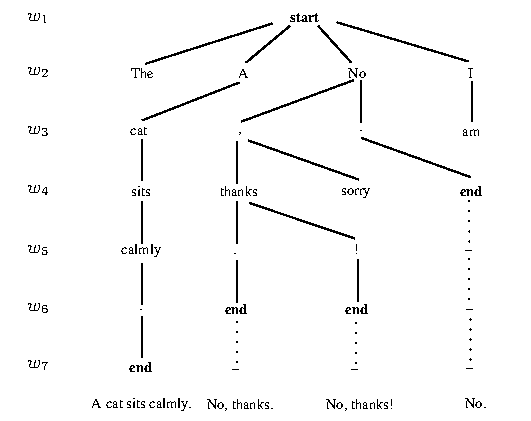
\includegraphics[width=\textwidth]{chapter2/img/bs.eps}
  \caption{\small{Hipotetyczny przykład działania algorytmu \textit{beam search} dla wiązki o rozmiarze 4. Dla przejrzystości w każdym kroku zaznaczono tylko elementy zawarte w wiązce.}}
\end{figure}

%!TEX output_directory = texaux
%!TEX spellcheck
%!TEX root = ../main.tex

\setlength{\abovedisplayskip}{20pt}
\setlength{\belowdisplayskip}{20pt}

\chapter{Generowanie dialogu}\label{rozdzial3}

Dialog opisujemy jako ciąg $U_1, U_2, \dots, U_K$ wypowiedzi w języku naturalnym. Każda wypowiedź jest sekwencją słów. Tak jak poprzednio korzystamy ze znaczników $\mathbf{start}$ i $\mathbf{end}$. Naginając nieco zapis:
\[U_k = {w_k}_1^{T_k} = (\mathbf{start}={w_k}_1, {w_k}_2, {w_k}_3, \dots, {w_k}_{T_k}=\mathbf{end})\]

\noindent
Rozszerzając przypadek pojedynczych sekwencji, możemy napisać
\[
\begin{aligned}
\hat{P}(U_1^K) &= \prod\limits_{k=1}^K \hat{P}(U_k \mid U_1^{k-1}\, ;\, \theta)\\
               &= \prod\limits_{k=1}^K \prod\limits_{t=1}^{T_k}
                  \hat{P}({w_k}_t \mid {w_k}_1^{t-1}, U_1^{k-1}\, ;\, \theta)
\end{aligned}
\]

Możemy wykorzystać \textit{RNNLM} do modelowania dialogu konkatenując poszczególne wypowiedzi. Otrzymany ciąg $U_1^\frown U_2^\frown \cdots^\frown U_K$ traktujemy jak jedną sekwencję. Niekoniecznie jest to jednak najlepsza metoda. W dalszej części rozdziału przedstawię opisany w \cite{serbanhred} model, który radzi sobie trochę lepiej. Pokażę też, jak wyglądały dialogi generowane przez moją implementację.

%%%%%%%%%%%%%%%%%%%%%%%%%%%%%%%%%%%%%%%%%%%%%%%%%%%%%%%%%%%%%%%%%%%%%%%%%

\section{Dostępność danych}

Zanim przystąpimy do optymalizacji modeli, trzeba zdobyć materiał uczący. Znalezienie dużej liczby publicznie dostępnych tekstów, szczególnie w języku angielskim, nie stanowi ogromnego problemu, nawet dla pojedynczych osób. Wszystkie artykuły Wikipedii są regularnie udostępniane w wygodnym formacie w postaci możliwych do pobrania zrzutów. Common Crawl\footnote{\url{http://commoncrawl.org/}} daje możliwość analizy zawartości blisko 3 miliardów stron internetowych. Dzieła literackie, archiwa gazet, cyfrowe zbiory bibliotek, ze wszystkich tych źródeł można korzystać za darmo.

Jeśli chcemy jednak znaleźć dane dialogowe mogące posłużyć do trenowania chatbota, sprawy mają się nieco inaczej. Duże zbiory danych istnieją, ale tym, z~którymi się spotkałem, sporo brakuje do statusu idealnego źródła.

\begin{itemize}
    \item \textbf{MovieTriples} \cite{serbanhred}\\[3pt]
    Zbiór napisów filmowych. W jego skład wchodzi 250\,000 trójek wypowiedzi. Każda trójka stanowi spójny fragment większego dialogu. Dane są udostępniane przez autorów na życzenie.

    \item \textbf{SubTle} \cite{subtle}\\[3pt]
    Kolejny, większy zbiór napisów do filmów. Gromadzi skrypty 5\,764 filmów, co przekłada się na 5,5 miliona pełnych tur dialogowych, czyli par kolejnych wypowiedzi. Podobnie jak \textit{MovieTriples}, dostępny na życzenie.

    \item \textbf{Ubuntu Dialogue Corpus} \cite{ubuntu}\\[3pt]
    Około 1 miliona dialogów dotyczących problemów technicznych nękających użytkowników Ubuntu. Korpus jest publicznie dostępny\footnote{\url{https://irclogs.ubuntu.com/}}.

    \item \textbf{\st{Twitter}} \cite{snapdata}\\[3pt]
    Do niedawna Uniwersytet Stanforda udostępniał kolekcję tweetów z drugiej połowy 2009 roku. Liczyła ona 467 milionów wiadomości. Niestety na prośbę Twittera zbiór musiał zostać usunięty z Internetu.

    \item \textbf{Reddit}\\[3pt]
    Istnieje możliwość pobrania liczącego setki gigabajtów zrzutu\footnote{\url{https://bigquery.cloud.google.com/dataset/fh-bigquery:reddit_comments}} komentarzy z~forum Reddit\footnote{\url{https://www.reddit.com/}}.
\end{itemize}

Problemem tych zbiorów danych jest bardzo silne zanurzenie w kontekście. Fakt ten czyni zadanie przewidywania odpowiedzi bardzo trudnym, nawet dla człowieka. Podejmujemy się zadania modelowania dialogu na podstawie samego tekstu, podczas gdy wypowiedzi uczestników rozmowy są podyktowane także innymi czynnikami. W przypadku filmów na zrozumienie przekazu składają się nie tylko wymiany zdań bohaterów, lecz także ton ich głosu, gestykulacja, sytuacja, w której się znajdują, czy wreszcie cała reszta filmu, którą widz zna, a o której sieć neuronowa nie ma pojęcia.

\textit{Ubuntu Dialogue Corpus} ma tę zaletę, że zapisy rozmów zawierają wszystkie niezbędne informacje. Użytkownicy komunikują się tylko za pomocą tekstu, a problem, z~którym się zmagają, jest opisany w rozmowie. To daje osobie zaznajomionej z~tematem możliwość pełnego zrozumienia dialogu. Wadą tych danych natomiast jest ich tematyka. Rozwiązywanie problemów technicznych wymaga dogłębnej wiedzy i~umiejętności wnioskowania, której maszyna czytająca forum się nie nauczy. O ile, choć z trudem, można wyobrazić sobie robota powtarzającego zapamiętane odpowiedzi na najczęściej pojawiające się pytania, o tyle przydatność chatbota w~analizie jakiegokolwiek niestandardowego zjawiska byłaby znikoma. Z drugiej strony dane zawierają wyłącznie rozmowy techniczne, więc robot będzie korzystał z dość hermetycznego języka informatycznego. Jeśli zadamy sobie pytanie: o czym taki program miałby rozmawiać?, to wszystko wydaje się prowadzić do sprzecznych celów.

Tweety również nie są zawieszone w próżni. Zwykle stanowią komentarz do wydarzenia znanego przynajmniej jednej ze stron, często mają charakter informacyjny. Czasami łączą się w krótkie rozmowy, co połączone z limitem 140 znaków daje pewne nadzieje, ale niestety nie miałem okazji tego sprawdzić.

Reddit nie posiada ograniczenia długości wiadomości. Powoduje to konieczność odfiltrowania rozmów, w których pojawiają się długie wypowiedzi; w przypadku czatu nie miałyby one racji bytu. Poza tym każdy wątek na Reddicie jest osadzony w kontekście, który stanowi pierwszy post. Raczej rzadko bywa to po prostu krótkie pytanie ogólne. Kontekst może być dość konkretnym tekstem, linkiem, często nawet obrazkiem lub filmem, co sprawia, że przewidywanie odpowiedzi bez niego staje się wręcz niemożliwe.

Swoje implementacje uczyłem na \textit{MovieTriples} i \textit{SubTle}. Z jednej strony dlatego, że były one wykorzystane w \cite{serbanhred}, więc wynik na nich stanowiłby dla mnie weryfikację poprawności kodu. Z drugiej strony są one względnie małe, więc proces uczenia modeli był na tyle krótki, że mogłem go wielokrotnie powtarzać.

%%%%%%%%%%%%%%%%%%%%%%%%%%%%%%%%%%%%%%%%%%%%%%%%%%%%%%%%%%%%%%%%%%%%%%%%%

\section{Model hierarchiczny}
Ta sekcja stanowi opis wykorzystanej w \cite{serbanhred} hierarchicznej architektury rekurencyjnej (ang. \textit{Hierarchical Recurrent Encoder-Decoder, HRED}) \cite{hred} do modelowania dialogu.

Oryginalnie \textit{HRED} miał służyć do przewidywania haseł, które użytkownik może wpisać w wyszukiwarce. Mechanizm zgadujący zapytania miał brać pod uwagę historię wyszukiwania, która mogła być dowolnie długa. Autorzy proponują podejście dwuetapowe: potraktować każde zapytanie jako osobną sekwencję, a całą historię jako ciąg zapytań. Ułatwi to sieci znajdowanie zależności pomiędzy całymi hasłami poprzez zredukowanie liczby kroków obliczeń mających miejsce między początkami dwóch kolejnych ciągów.

%%%%%%%%%%%%%%%%%%%

\subsection{Architektura \textit{encoder-decoder}}
W poprzednim rozdziale tekst generowany za pomocą \textit{RNNLM} miał przypominać tekst wejściowy. Generator był nie tylko deterministyczny, ale również w żaden sposób nie uwarunkowany. Wynik zależał wyłącznie od $\theta$ i od początkowego stanu sieci rekurencyjnej, $h_0$. Niektóre zastosowania wymagają generowania sekwencji zupełnie odmiennych od tekstu wejściowego, ale w pewien sposób z nim powiązanych. Za przykład niech posłuży tłumaczenie maszynowe, gdzie na podstawie zdania w~jednym języku chcemy, zachowując znaczenie, wyprodukować zdanie w drugim. Załóżmy, że chcemy uzależnić model od pewnego warunku początkowego $A$:
\[P(w_1^T) = \prod\limits_{t=1}^T P(w_t \mid w_1^{t-1}, A)\]

Odpowiednia modyfikacja \textit{RNNLM} pozwala osiągnąć ten cel. Zachowaniem generatora można sterować poprzez zmianę $h_0$. Wystarczy, że będziemy potrafili zakodować $A$ jako pewne $a \in \mathbb{R}^m$, gdzie $m$ jest wymiarem stanu sieci rekurencyjnej. Wówczas pozostaje tylko ustawić $h_0 := a$.

W przypadku pracy z tekstem, warunkiem początkowym będzie oczywiście jakaś sekwencja słów $A = a_1^{T_a}$. Żeby ją zakodować w $\mathbb{R}^m$ możemy wykorzystać drugą sieć rekurencyjną. Oznaczmy jej kolejne stany przez $s_1^{T_a}$. Można myśleć, że $s_i$ jest podsumowaniem sekwencji $a_1^i$. Ponieważ reprezentacją $A$ ma być pojedynczy wektor, będzie nas interesował wyłącznie ostatni stan. Ciąg $A$ kodujemy jako $s_{T_a}$.

Mamy więc dwa ciągi wejściowe: źródłowy $a_1^{T_a}$ i docelowy $w_1^T$. Zmodyfikowana architektura wygląda tak:
\begin{enumerate}
    \item \textbf{Warstwa zanurzeń}: identyczna jak w \textit{RNNLM}, ale zanurzamy obie sekwencje. Warstwa przerabia $a_1^{T_a}$ na ciąg wektorów $x_1^{T_a}$ oraz $w_1^T$ na $y_1^T$.
    \item \textbf{Kodujący \textit{RNN}}: przechodzi po $x_1^{T_a}$ i oblicza $s_{T_a}$.
    \item \textbf{Dekodujący \textit{RNN}}: czyta $y_1^T$ i produkuje ciąg stanów $h_1^T$, startując ze stanu początkowego $h_0 = s_{T_a}$.
    \item \textbf{Softmax}: tak jak w \textit{RNNLM}, $h_0^{T-1}$ jest przekształcane na ciąg $p_1^T$ rozkładów prawdopodobieństwa na $V$, tym razem zależnych od $A$.
\end{enumerate}

\begin{figure}[ht]
  \centering
    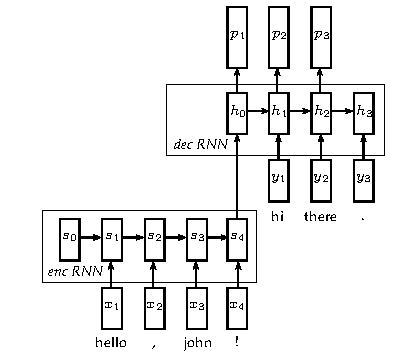
\includegraphics[width=0.8\textwidth]{chapter3/img/encdec.eps}
  \caption{\small{Przetwarzanie pary dialogowej przez \textit{encoder-decoder}. Dla czytelności warstwa zanurzeń została pominięta.}}
\end{figure}

Podobnie jak w \textit{RNNLM}, optymalizujemy parametry minimalizując \textit{nll} na ciągu docelowym, czyli
\[-\sum\limits_{t=1}^T \ln((p_t)_{w_t}).\]

Modele uczące się zależności pomiędzy parami ciągów, są w literaturze określane jako \textit{sequence-to-sequence}, lub w skrócie \textit{seq2seq}. Ze względu na swoją konstrukcję, ta sieć nosi również nazwę \textit{encoder-decoder}. Pomysł ten, w wersji gęstej, został po raz pierwszy przedstawiony już w 1997 roku \cite{encdecfirst}. Współczesny wariant rekurencyjny zawdzięcza swoją popularność m.in. dobrym wynikom w~zadaniu tłumaczenia maszynowego \cite{encdec}.

%%%%%%%%%%%%%%%%%%%

\subsection{Hierarchiczny rekurencyjny \textit{encoder-decoder}}
Przypomnijmy, że dialogiem jest ciąg $U_1^K$, gdzie $U_k = {w_k}_1^{T_k}$. \textit{HRED} wykorzystuje architekturę \textit{seq2seq}. Modelowanie rozmowy jest w końcu zadaniem przekształcania sekwencji. Istotna różnicę stanowi jednak fakt, że w dialogu wypowiedź $U_k$ zależy od wszystkich poprzednich wypowiedzi. Ciągów docelowych jest zatem więcej, ponieważ wygenerowanie $U_k$ stanowi nasz cel po przeczytaniu $U_1^{k-1}$. Pojawia się naturalna hierarchia: poziom słów i poziom zdań.

Na poziomie słów wypowiedzi są zwijane do pojedynczych wektorów. Na poziomie zdań ciąg reprezentacji wypowiedzi jest analogicznie kodowany jako wektor. Później do akcji wkracza dekoder. Chcemy wykorzystać cały dialog do uczenia modelu, dlatego dekoder przechodzi po kolei po każdej z wypowiedzi. Zestaw parametrów dekodera jest tylko jeden, ale stan w każdym z tych przejść inicjowany jest inaczej. Kiedy dekoder zaczyna czytać $U_k$, jego stan początkowy zależy od wektora podsumowującego $U_1^{k-1}$. Po przetworzeniu całego $U_k$, produkowane są warunkowe rozkłady prawdopodobieństwa.

\noindent
Definicje funkcji $f$ i $g$ pojawiających się w poniższym opisie znajdują się dalej.
\begin{enumerate}
    \item \textbf{Warstwa zanurzeń}: każde $U_k$ jest zanurzane jako ${x_k}_1^{T_k}$.
    \item \textbf{\textit{RNN} poziomu 1 (kodujący zdania)}: dla każdego $k$ przechodzi po ${x_k}_1^{T_k}$ produkując podsumowanie sekwencji, $s_k$. Cały dialog teraz reprezentowany jest przez ciąg wektorów $s_1^K$.
    \item \textbf{\textit{RNN} poziomu 2 (kodujący kontekst)}: przechodzi po $s_1^K$ tworząc ciąg stanów $c_1^K$. Każde $c_k$ stanowi podsumowanie $U_1^k$, a $c_0$ = $\vv{0}$.
    \item \textbf{Dekodujący \textit{RNN}}: dla każdego $k$ przechodzi po ${x_k}_1^{T_k}$ produkując ciąg stanów ${d_k}_1^{T_k}$, zaczynając od ${d_k}_0 = f(c_{k-1})$.
    \item \textbf{Softmax}: tym razem przed wejściem do warstwy \textit{softmax}, do stanów dekodera dokładamy bezpośrednią informację o poprzedzającym słowie. Dla każdego $k \in \{1,\dots,K\}$ powstaje ciąg ${p_k}_1^{T_k}$ rozkładów na $V$. Rozkład ${p_k}_t$ jest obliczany na podstawie wektora $g(d_{k,t-1}, x_{k,t-1})$.
\end{enumerate}

\begin{figure}[ht]
  \centering
    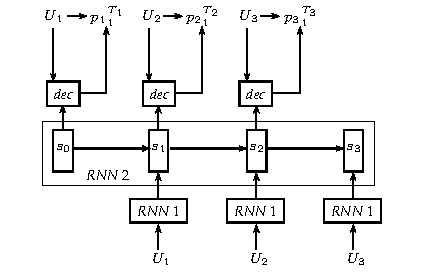
\includegraphics[width=0.9\textwidth]{chapter3/img/hred.eps}
  \caption{\small{Uproszczony schemat modelu hierarchicznego.}}
\end{figure}

Każde ${p_k}_t$ określa prawdopodobieństwa wystąpienia poszczególnych słów na $t$-tej pozycji w $U_k$, biorąc pod uwagę poprzednie wypowiedzi i słowa. Zgodnie z~założonym modelem probabilistycznym dostajemy
\[({p_k}_t)_{{w_k}_t} = \hat{P}({w_k}_t \mid {w_k}_1^{t-1}, U_1^{k-1}\, ;\, \theta).\]

\subsubsection{Szczegóły architektury}

Autorzy w dwóch miejscach korzystają z dodatkowych transformacji wyjścia sieci rekurencyjnej. Przy inicjowaniu stanu dekodera pojawia się warstwa afiniczna:
\[f(c) = \tanh(D_0 c + b_0)\]
Przy obliczaniu prawdopodobieństw akcentowany jest wpływ poprzedniego słowa:
\[g(d, x) = H_o d + E_o x + b_o\]

Sieci rekurencyjne wykorzystywane do kodowania wypowiedzi i dialogu są dwustronne (sekcja~\ref{birnn}). Końcowy stan jest konkatenacją norm $L_2$ nałożonych na ciągi stanów pośrednich. Powiedzmy, że chcemy złączyć ciągi $q_1^I$ i ${q_r}_1^I$, gdzie $\forall_i\ q_i \in \mathbb{R}^{m}$, ${q_r}_i \in \mathbb{R}^{m_r}$. Wynikiem będzie
\[
\begin{bmatrix}
    q\\
    q_r
\end{bmatrix} \in \mathbb{R}^{(m + m_r)},
\]
gdzie
\[
\begin{aligned}
    q &= \sqrt{\frac{1}{I} \sum_{i=1}^I (q_i)^2}\\[10pt]
    q_r &= \sqrt{\frac{1}{I} \sum_{i=1}^I ({q_r}_i)^2}
\end{aligned}
\]

\noindent
Działania pierwiastka i potęgowania są nakładane na każdy element wektora osobno.

\noindent
Cały mechanizm jest zatem parametryzowany przez następujące wartości:

Stałe:\vspace{-.3cm}
\begin{itemize}[leftmargin=1.5cm,label={\tiny$\bullet$}]
    \itemsep0em
    \item $V$ -- słownik
    \item $n$ -- rozmiar zanurzenia słowa
    \item $m_1$ -- rozmiar stanu \textit{RNN} poziomu 1
    \item $m_2$ -- rozmiar stanu \textit{RNN} poziomu 2
    \item $m_{dec}$ -- rozmiar stanu dekodera
    \item $m_{out}$ -- wymiar wejścia do warstwy \textit{softmax}
\end{itemize}

Optymalizowane:\vspace{-.3cm}
\begin{itemize}[leftmargin=1.5cm,label={\tiny$\bullet$}]
    \itemsep0em
    \item $E \in \mathbb{R}^{n \times |V|}$ -- macierz zanurzeń słów
    \item parametry warstw rekurencyjnych
    \item $D_0 \in \mathbb{R}^{m_{dec} \times m_2}$, $b_0 \in \mathbb{R}^{m_{dec}}$ -- parametry warstwy afinicznej obliczającej początkowy stan dekodera
    \item $H_o \in \mathbb{R}^{m_{out} \times m_{dec}}$, $E_o \in \mathbb{R}^{m_{out} \times n}$, $b_o \in \mathbb{R}^{m_{out}}$ -- parametry wiążące bezpośrednio stan dekodera z poprzednim słowem
\end{itemize}
\noindent
Uczymy sieć minimalizując \textit{nll} całego dialogu, czyli
\[-\sum\limits_{k=1}^K \sum\limits_{t=1}^{T_k} \ln(({p_k}_t)_{{w_k}_t}).\]

%%%%%%%%%%%%%%%%%%%%%%%%%%%%%%%%%%%%%%%%%%%%%%%%%%%%%%%%%%%%%%%%%%%%%%%%%

\section{Eksperymenty}
Dołączony kod zawiera moje implementacje \textit{RNNLM} i \textit{HRED}. Oba modele wykorzystują jednostki \textit{GRU} jako warstwy rekurencyjne. Uczenie ich było odtworzeniem procedury z \cite{serbanhred}. Mechanizmy zostały wytrenowane metodą \textit{ADAM} (sekcja~\ref{adam}) z wykorzystaniem podziału na zbiory uczący, testowy i walidacyjny (sekcja~\ref{testset}). Korzystałem z udostępnionych mi zbiorów danych \textit{MovieTriples} i \textit{SubTle}. Oprócz klasycznego \textit{softmaxa} wypróbowałem wersję próbkowaną (\ref{ssoft}) z rozmiarem próbki 200. Cały proces przebiegał w dwóch etapach:

\begin{enumerate}
    \item Inicjujemy losowo optymalizowalne parametry, łącznie z macierzą zanurzeń słów. Następnie uczymy je przez jakiś czas na \textit{SubTle}. Wykonujemy w~ten sposób kilka przebiegów po zbiorze uczącym, w tym przypadku 4.
    \item Otrzymany model dostrajamy na \textit{MovieTriples}. Ustalamy zanurzenia i optymalizujemy tylko pozostałe parametry. Moment przerwania algorytmu wybieramy przy pomocy \textit{early stopping} z $k=5$ (opisane w~\ref{earlys}).
\end{enumerate}
\noindent
Wartości $n$, $m_1$, $m_2$, $m_{dec}$, $m_{out}$ zostały ustawione na 300. Słownik $V$ liczył 10\,000 elementów, słowa nieznane zastąpiono tagiem $\mathbf{unk}$.

W Tabeli~\ref{hredtab} zamieszczam średnie wartości \textit{nll} na zbiorze testowym \textit{MovieTriples}, wraz z czasami potrzebnymi do wyuczenia modeli. Wydają się one lepsze od tych przedstawionych w \cite{serbanhred}, więc podejrzewam, że sposób mierzenia błędu może się nieco różnić. Zgodnie z oczekiwaniami \textit{HRED} sprawdził się lepiej od \textit{RNNLM}, chociaż różnica nie była duża. Próbkowany \textit{softmax} dwukrotnie przyspieszył proces uczenia, ale uzyskał wynik istotnie gorszy od pełnej wersji. Rozwiązanie to jednak dużo lepiej się skaluje, więc w przypadku większych danych (i słownika liczącego setki tysięcy pozycji) zaoszczędzony czas moglibyśmy mierzyć w dniach, a~nawet tygodniach.

\setlength{\tabcolsep}{3pt}
\begin{table}[H]
    \centering
    \caption{Wyniki modeli na zbiorze testowym}
    \label{hredtab}
    \begin{tabular}{|l|r|r|}
        \hhline{~--}
        \multicolumn{1}{c|}{} & \cellcolor[gray]{.85}\textbf{Softmax pełny} & \cellcolor[gray]{.85}\textbf{Softmax próbkowany}\\
        \hline
        \cellcolor[gray]{.85}\textbf{RNNLM} & \makecell[r]{3.197\\14.3h} & \makecell[r]{3.223\\7.4h} \\
        \hline
        \cellcolor[gray]{.85}\textbf{HRED} & \makecell[r]{3.192\\23.5h} & \makecell[r]{3.205\\11.9h} \\
        \hline
    \end{tabular}\par
\end{table}

%%%%%%%%%%%%%%%%%%%

\subsection{Generowanie wypowiedzi}

Automatyczne ocenianie jakości generowanego dialogu jest trudnym zadaniem. Autorzy \cite{hownotto} zauważają że, popularne metody ewaluacji dość słabo korelują z osądem człowieka. Decyzję o tym, czy model daje dobre wyniki podejmowałem więc przez prostą obserwację przykładów. Metoda ``na oko'' ma swoje wady, ale pozwala zauważyć pewne zachowania właściwe różnym ustawieniom generatora.

W tym fragmencie pracy przedstawiam przykłady wygenerowanych dialogów oraz kilka modyfikacji algorytmu, które mogą poprawić ich jakość. Korzystam z modelu \textit{HRED} i~pełnego \textit{softmaxa}. Dialogi otrzymane za pomocą \textit{RNNLM} wyglądały bardzo podobnie. Na początek rozmowa uzyskana najprostszym algorytmem. Działa on według opisu z sekcji~\ref{gen}, z tą różnicą, że podczas przygotowywania odpowiedzi sieć bierze pod uwagę kontekst konwersacji w sposób przedstawiony na początku rozdziału~\ref{rozdzial3}\\

%!TEX output_directory = texaux
%!TEX spellcheck
%!TEX root = ../main.tex

\setlength{\abovedisplayskip}{20pt}
\setlength{\belowdisplayskip}{20pt}

\small

\textbf{U}: Hello!\\\indent
\textbf{B}: Hi.\\\indent
\textbf{U}: How are you?\\\indent
\textbf{B}: I'm fine.\\\indent
\textbf{U}: Do you want to eat something?\\\indent
\textbf{B}: No.\\\indent
\textbf{U}: Why not?\\\indent
\textbf{B}: I don't know.\\\indent
\textbf{U}: I guess you are not hungry?\\\indent
\textbf{B}: No.\\\indent
\textbf{U}: OK. I will leave you now.\\\indent
\textbf{B}: No.\\

\normalsize

Odpowiedzi można opisać jako bardzo zdawkowe. Zwykle pasują gramatycznie do kontekstu, ale nic konkretnego do rozmowy nie wnoszą. Spójrzmy na listę propozycji ostatniej odpowiedzi bota, wraz z ocenami ich jakości:\\

\small
-4.116 \ no .\\\indent
-4.305 \ what ?\\\indent
-5.035 \ yes .\\\indent
-5.370 \ why ?\\\indent
-5.608 \ please .\\\indent
-6.124 \ i will .\\\indent
-6.815 \ what are you doing ?\\\indent
-6.890 \ what do you want ?\\\indent
-6.965 \ i can ' t .\\\indent
-7.018 \ i ' m sorry .\\
\normalsize

Bardzo krótkie wypowiedzi mają najwyższe wyniki i są preferowane przez generator. W dużej mierze wiąże się to z ich uniwersalnością. Wolelibyśmy jednak, żeby bot wyrażał się mniej lakonicznie. Można na przykład premiować dłuższe sekwencje przez dodawanie arbitralnego bonusu zależnego od długości. Bardziej eleganckim sposobem wydaje się jednak uśrednienie wyniku po wszystkich słowach.\\

%!TEX output_directory = texaux
%!TEX spellcheck
%!TEX root = ../main.tex

\setlength{\abovedisplayskip}{20pt}
\setlength{\belowdisplayskip}{20pt}

\small
\textbf{U}: Hi!\\\indent
\textbf{B}: What are you doing here?\\\indent
\textbf{U}: I am working on my thesis\\\indent
\textbf{B}: I don't know what you're talking about.\\\indent
\textbf{U}: I try to make a robot speak.\\\indent
\textbf{B}: I don't know what you're talking about.\\\indent
\textbf{U}: What do you know then?\\\indent
\textbf{B}: I don't know.\\\indent
\textbf{U}: Are you OK?\\\indent
\textbf{B}: I'm fine.\\\indent
\textbf{U}: Can we talk a bit?\\\indent
\textbf{B}: I don't know what you're talking about.\\
% \textbf{U}: \\\indent
% \textbf{B}: \\
% \textbf{U}: \\\indent
% \textbf{B}: \\

\normalsize

Robot nagle stał się szczery do bólu. Widać jednak, że korzysta również z dłuższych sekwencji, co potwierdza nowy ranking propozycji. Wyniki są też bardziej zrównoważone.\\

\small
-0.844 \ i don ' t know what you ' re talking about .\\\indent
-0.855 \ i ' m fine .\\\indent
-0.856 \ i don ' t know .\\\indent
-0.907 \ i don ' t want to talk about it .\\\indent
-0.926 \ i don ' t think so .\\\indent
-0.929 \ no , i ' m fine .\\\indent
-0.949 \ no .\\\indent
-0.989 \ i don ' t know what to say .\\\indent
-1.014 \ sure .\\\indent
-1.028 \ i don ' t want to talk about this .\\
\normalsize

Niestety system często zwraca generyczne odpowiedzi, które gramatycznie pasują do wielu kontekstów. Bardzo trudno byłoby odsiać wypowiedzi ogólnikowe od konkretów (najpierw trzeba by potrafić to zrobić ręcznie, a nawet to nie jest oczywiste). Poza tym nie chcemy całkowicie zakazać odpowiedzi typu \textit{I don't know}. Możemy jednak sprawić, żeby model korzystał z nich rzadziej, przez wprowadzenie losowości do dialogu.

Istnieją dwa miejsca, w których generator wybiera najlepiej oceniany element. Podczas budowania listy propozycji algorytmem przeszukiwania wiązkowego słowa z~największym prawdopodobieństwem są doklejane do już istniejących sekwencji. Kiedy lista jest gotowa, zwracana jest odpowiedź z najwyższym wynikiem. Oba te procesy można poddać randomizacji: zamiast brać ``najlepszy'' element, losować zwycięzcę. Żeby wyraźnie odróżnić słabe możliwości od lepszych, prawdopodobieństwa wyboru poszczególnych elementów wykładniczo zależą od ich ocen. Dodając do tego normalizację otrzymujemy funkcję \textit{softmax}. Stosując dodatkowe potęgowanie możemy ją wyostrzać lub wygładzać, co pozwala sterować stopniem losowości.

Randomizacja wyboru pełnych wypowiedzi znacznie zmienia naturę generatora. Dialogi stają się bardziej różnorodne i ciekawsze, chociaż niezrozumienie kontekstu pozostaje. Problem powtarzania uniwersalnych zdań nie został wyeliminowany. Konwersacje nabierają jednak wartości rozrywkowej, co w obliczu nudnych alternatyw przedstawionych powyżej przemawia za tym rozwiązaniem. Losowanie pojedynczych słów na etapie przeszukiwania również wydaje się wprowadzać pożądaną różnorodność, chociaż bardziej subtelnie. Poniżej przykład z włączonymi obiema opcjami.\\

%!TEX output_directory = texaux
%!TEX spellcheck
%!TEX root = ../main.tex

\setlength{\abovedisplayskip}{20pt}
\setlength{\belowdisplayskip}{20pt}

\small
\textbf{U}: Good morning.\\\indent
\textbf{B}: I'll see you in the morning, okay?\\\indent
\textbf{U}: Can't we talk now?\\\indent
\textbf{B}: I don't want to talk about this anymore.\\\indent
\textbf{U}: Tell me what's wrong.\\\indent
\textbf{B}: I don't know what you're talking about. It's not that simple. It's a lot of things to\\\indent\indent get.\\\indent
\textbf{U}: What do you want to get?\\\indent
\textbf{B}: I don't know. It's a lot of money. What do you want me to do?\\\indent
\textbf{U}: You are not talking about robbery, are you?\\\indent
\textbf{B}: I don't know what you're talking about. It's not your fault.\\\indent
\textbf{U}: I am relieved.\\\indent
\textbf{B}: It's not your fault. You're just trying to get me out of the way.\\\indent
\textbf{U}: I would never do such a thing!\\\indent
\textbf{B}: You don't have to know what I'm talking about. It's not gonna happen, right?\\\indent
\textbf{U}: I think you should tell me your plans.\\\indent
\textbf{B}: I don't want to talk about it. I'm not going to go out with you. I'm gonna be okay.\\\indent
\textbf{U}: Whatever. Bye then.\\\indent
\textbf{B}: I don't know what you're talking about. It's been a while since I was a kid, but I'm\\\indent\indent not going to be able to tell you the truth. I've never done anything like that.\\
% \textbf{U}: \\\indent
% \textbf{B}: \\\indent

\normalsize

Jest znacznie lepiej, chociaż niektóre wypowiedzi są zdecydowanie za długie. System wciąż nie wie o czym mówi, do czego zresztą sam często się przyznaje. Tego problemu nie wyeliminowałem, ale jedno usprawnienie jeszcze udało się zrobić. Przyjrzyjmy się liście propozycji:\\

\small
-1.205 \ it ' s not your fault .\\\indent
-1.408 \ you don ' t believe me .\\\indent
-1.415 \ you don ' t believe me ?\\\indent
-1.423 \ it ' s not your fault . i can ' t get you out of here .\\\indent
-1.453 \ it ' s not your fault !\\\indent
-1.464 \ it ' s not your fault . i can ' t get you out of this .\\\indent
-1.482 \ it ' s not your fault . i can ' t get you out of the way .\\\indent
-1.509 \ it ' s not your fault . you ' re just trying to get me out of the way .\\\indent
-1.533 \ it ' s your fault .\\\indent
-1.536 \ it ' s not your fault . you know how to do this ?\\
\normalsize

Okazuje się, że jest ona zdominowana przez mało różniące się od siebie wypowiedzi. Taka jest niestety natura przeszukiwania wiązkowego. Wczesna homogenizacja wiązki blokuje innowacje w przyszłości. Autorzy \cite{dbs} próbują obejść to zjawisko. Rezultatem jest algorytm zróżnicowanego przeszukiwania wiązkowego (ang. \textit{Diverse Beam Search}, dalej \textit{DBS}).

\subsubsection{\textit{Diverse Beam Search}}

W algorytmie \textit{DBS} wiązka jest podzielona na wiele mniejszych wiązek (grup). W każdej z nich przeprowadzane jest normalne przeszukiwanie wiązkowe, z jedną tylko różnicą: prawdopodobieństwa słów występujących na aktualnej pozycji w poprzednich grupach są sztucznie zmniejszane. W ten sposób każda grupa stara się odróżniać od pozostałych omijając użyte już wyrazy. Wartość kary można uzależnić od liczby wystąpień danego słowa. Zastosowanie podziału na wąskie ścieżki powoduje, że homogenizacja następuje na poziomie grup, ale cała wiązka zawiera różnorodne ciągi. Oczywiście po wprowadzeniu tej modyfikacji wartości dla poszczególnych słów nie sumują się do 1, więc przestajemy mieć do czynienia z rozkładem.

Stosując \textit{DBS} trzeba dobrze wybrać rozmiar grupy. Małe liczby dają większą różnorodność, ale i mniej składne wypowiedzi. Zauważyłem też, że dialogi wyglądają sensowniej po wyłączeniu randomizacji wyboru pojedynczych słów. Mały rozmiar wiązki w połączeniu z losowością dawał czasem dość bezsensowne odpowiedzi.
\\[1cm]
\begin{algorithm}[H]
    \SetAlgorithmName{Algorytm}
    \\\\$K$ -- szerokość wiązki\\
    $G$ -- liczba grup\\
    $z$ -- kara dla już występujących słów\\[5pt]
    $g = K / G$ -- rozmiar grupy\\
    \For{$i \gets 2$ \KwTo $G$}{
        $beam^i$ -- $i$-ta grupa, inicjowana jako $\{((\mathbf{start}), 0)\}$
    }
    $beam \gets (beam^1, beam^2,\dots, beam^G)$\\
    \While{\textnormal{istnieją niezakończone ciągi w elementach} $beam$}{
        \For{$i \gets 1$ \KwTo $G$}{
            $cont^i \gets \{\}$\\
            \For{$(seq,\ scr) \mathbf{\ in\ } beam^i$}{
                $S \gets \bigcup_{j<i}$ \{słowa występujące na końcach ciągów w $beam^j$\}\\
                \For{$v \mathbf{\ in\ } V$}{
                    $p_{log} \gets \ln(\hat{P}(v \mid seq\, ;\, \theta_{opt}))$\\
                    \If{$v \in S$}{
                        $p_{log} \gets p_{log} - z$\\
                    }
                    $cont \gets cont \cup \{(seq^\frown (v),\ scr + p_{log})\}$
                }
            }
            $beam^i \gets$ podzbiór $g$ elementów $cont$ o najwyższych wynikach
        }
        $beam \gets (beam^1, beam^2,\dots, beam^G)$\\
    }
    \Return $beam$
    \caption{Diverse Beam Search}
\end{algorithm}

\vspace{1cm}

\noindent
Poniżej przykład zabawnej rozmowy, w której stosuję \textit{DBS} dla $K=20$ i $g=2$.\\

%!TEX output_directory = texaux
%!TEX spellcheck
%!TEX root = ../main.tex

\setlength{\abovedisplayskip}{20pt}
\setlength{\belowdisplayskip}{20pt}

\small
\textbf{U}: I like summer.\\\indent
\textbf{B}: And I don't know what you mean, but I think it's a good thing to do with\\\indent\indent your own life.\\\indent
\textbf{U}: Poor robot, you never saw summer...\\\indent
\textbf{B}: I don't know what to say. But it's not like that. It's just a dream sequence.\\\indent
\textbf{U}: You can have dreams?\\\indent
\textbf{B}: Not yet. It's just a dream sequence, and I've never seen anything like that before.\\\indent\indent But I'm afraid of you, I don't know what to do with this.\\\indent
\textbf{U}: I will teach you about the world.\\\indent
\textbf{B}: Oh, yes. I'm sorry, but I have to go back and see if you can help me out of the way\\\indent
\textbf{U}: No, wait! Don't go!\\\indent
\textbf{B}: I'm not going anywhere. I'll be back in a minute, but we're not gonna do anything\\\indent\indent about it! We can't go to the police!\\\indent
\textbf{U}: I never mentioned the police\\\indent
\textbf{B}: Then why?! You're not going to be able to get out of this, but it'snot your fault.\\\indent
\textbf{U}: Am I in trouble?\\\indent
\textbf{B}: It's okay, I'm fine.\\\indent
\textbf{U}: Good to hear. I think I will go now.\\\indent
\textbf{B}: Why don't you go to bed and sleep with me. I'll be back in a minute.\\\indent
\textbf{U}: You are a robot, you know that?\\\indent
\textbf{B}: Yes, sir. I'm a little confused. I've been thinking about you, but it's not that simple. \\\indent
\textbf{U}: Definitely.\\\indent
\textbf{B}: Well, it's a lot of fun. I don't know what to do with the money. but I'm not going\\\indent\indent to be able to get you out of this house.\\

\normalsize

\subsubsection{Problemy i wnioski}

W przedstawionych przykładach generator miał ograniczony kontekst: brał pod uwagę tylko dwie ostatnie wypowiedzi. Włączenie nieograniczonej pamięci nie przyniosło wyraźnej poprawy, być może dlatego, że model był uczony tylko na trójkach. Długi kontekst połączony z \textit{DBS} i małym rozmiarem grupy daje jeszcze gorszy rezultat. Odpowiedzi po pewnym czasie zupełnie traciły sens. Jest to jeden z dwóch głównych problemów systemu. Przyczyna tkwi na pewno po części w rozmiarze danych. Rozmowy w zbiorze uczącym były bardzo krótkie i nie było ich wiele.

Drugi problem wydaje się trudniejszy, ale i ciekawszy, ponieważ dotyczy samej istoty modelowania dialogu na podstawie danych. Jest nim brak różnorodności w generowanych rozmowach. Należy zwrócić uwagę na fakt, że, niezależnie od rozmiaru danych, pewne wypowiedzi są bardzo uniwersalne, co czyni je dobrymi kandydatami w wielu sytuacjach. Zauważmy też, że dane uczące zawierają wypowiedzi osób o różnych charakterach i zachowaniach. W efekcie model nie posiada konkretnej osobowości, ale jest jednolitym zlepkiem wszystkiego, co usłyszał. Posługuje się uśrednionym stylem, nie posiada żadnych wyróżniających cech, a jego odpowiedzi są bardzo zachowawcze. To znacznie utrudnia generowanie różnorodnych wypowiedzi i~wprowadza konieczność modyfikacji prawdopodobieństw zwracanych przez model. Istnieje również problem samego oceniania jakości otrzymywanych dialogów \cite{hownotto}, co sprawia, że trudno sprawdzić, czy konkretne zmiany w generatorze faktycznie go poprawiają. Nie mamy nawet pewności, czy maksymalizowanie wiarygodności jest faktycznie najlepszym sposobem uczenia \cite{serbanhred}.

Myślę, że znacznie łatwiejsze byłoby modelowanie dialogów, w których jedną ze stron jest zawsze ta sama osoba. Wówczas odpowiedzi w powtarzających się sytuacjach byłyby podobne, co daje nadzieję na nauczenie się konkretnych zachowań. Niestety obecnie zgromadzenie odpowiedniej ilości takich danych byłoby niezwykle trudne, więc pomysł jest czysto hipotetyczny.

%!TEX output_directory = texaux
%!TEX spellcheck
%!TEX root = ../main.tex

\setlength{\abovedisplayskip}{20pt}
\setlength{\belowdisplayskip}{20pt}

\chapter{Odpowiadanie na pytania} \label{rozdzial4}

Poprzednio opisane mechanizmy budowały model ogólnej rozmowy. Bot był bardzo ograniczony w swojej umiejętności rozumienia tekstu. Jego odpowiedzi co prawda zwykle pasowały do kontekstu, ale niewiele więcej można o nich powiedzieć. Większość systemów dialogowych powstaje z myślą o konkretnym celu, do którego zrealizowania nie wystarczy prowadzenie ``rozmowy o niczym''. Użyteczny robot może na przykład być w~stanie dostarczyć człowiekowi wartościowych informacji. W tym rozdziale przedstawiam kolejne wyzwanie chatbotów, które może być rozwiązane za pomocą sieci neuronowej.

Chcemy nauczyć program odpowiadania na pytania o fakty formułowane w~języku naturalnym. Przykładem może być \textit{When was Battle of Grunwald?}. Sama analiza występowania słów tutaj nie wystarczy, musimy zaopatrzyć model w jakieś źródło wiedzy. Tym źródłem będzie krótki tekst w języku naturalnym. Naszym celem jest sprawić, by bot na powyższe pytanie odpowiedział poprawnie po przeczytaniu tekstu, który może wyglądać tak:\\

\small\textit{The Battle of Grunwald, First Battle of Tannenberg or Battle of Žalgiris, was fought on 15 July 1410 during the Polish–Lithuanian–Teutonic War. The alliance of the Kingdom of Poland and the Grand Duchy of Lithuania, led respectively by King Władysław II Jagiełło (Jogaila) and Grand Duke Vytautas, decisively defeated the German–Prussian Teutonic Knights, led by Grand Master Ulrich von Jungingen.}\footnote{Fragment pochodzi z \url{https://en.wikipedia.org/wiki/Battle_of_Grunwald}}\\

\normalsize
Powyższy problem cieszy się rosnącym zainteresowaniem wśród społeczności zajmujących się uczeniem maszynowym. W 2016 roku opublikowany został \textit{Stanford Question Answering Dataset (SQuAD)} \cite{squaddata}, zbiór danych zawierający blisko 86\,000 pytań. Do każdego pytania dołączony jest krótki fragment stanowiący kontekst. Skuteczność na \textit{SQuAD}zie jest popularną miarą jakości systemów odpowiadających na pytania o fakty. W ostatnim czasie najlepsze z nich niemalże dorównały umiejętnościom człowieka\footnote{\url{https://rajpurkar.github.io/SQuAD-explorer/}}.

W momencie przygotowywania tej pracy jedno z czołowych miejsc w rankingu \textit{SQuAD} zajmował system \textit{FastQA} \cite{fastqa}. Dalsza część rozdziału zawiera opis, przykłady zastosowania, i przedstawienie próby usprawnienia tego systemu.

%%%%%%%%%%%%%%%%%%%%%%%%%%%%%%%%%%%%%%%%%%%%%%%%%%%%%%%%%%%%%%%%%%%%%%%%%

\section{FastQA}

Jak wiele innych modeli tego typu, \textit{FastQA} odpowiada cytując pewien podciąg kontekstu. Dla każdego pytania $q = q_1^{K_q}$ w zbiorze uczącym mamy odpowiadający mu tekst $x = x_1^{K_x}$ oraz parę indeksów $\mathbf{s}, \mathbf{e} \in \{1,\dots,K_x\}$ takich, że $x_{\mathbf{s}}^{\mathbf{e}}$ jest poprawną odpowiedzią. Ucząc model staramy się maksymalizować prawdopodobieństwo wybrania właściwego ciągu, czyli
\[\hat{P}_s(\mathbf{s} \mid q, x)\ \hat{P}_e(\mathbf{e} \mid \mathbf{s}, q, x).\]

%%%%%%%%%%%%%%%%%%%

\subsection{Architektura sieci}

Podstawowy pomysł polega na zakodowaniu pytania i kontekstu za pomocą sieci rekurencyjnej, a następnie wykorzystaniu uzyskanej informacji do obliczenia $P_s$,~$P_e$~--~rozkładów prawdopodobieństwa na $\{1,\dots,K_x\}$. Można zrealizować go tak:

\begin{enumerate}
    \item \textbf{Zanurzenia}: zanurzamy $q$ jako $v_1^{K_q}$ i $x$ jako $u_1^{K_x}$.
    \item \textbf{Kodujący \textit{RNN}}: zamieniamy $v_1^{K_q}$ na ciąg wektorów $z_1^{K_q}$ oraz $u_1^{K_x}$ na $h_1^{K_x}$.
    \item \textbf{Reprezentacja pytania}: w pewien sposób agregujemy ciąg $z_1^{K_q}$ do jednego wektora $\tilde{z}$ reprezentującego pytanie.
    \item \textbf{Początki}: do każdego $h_i$ dodajemy informację o $\tilde{z}$, aby powiązać pytanie z~kontekstem. Powstaje ciąg ${h'}_1^{K_x}$. Wektory $h'_i$ są zwijane do skalarów. Funkcja \textit{softmax} nałożona na wynik daje prawdopodobieństwa $\hat{P}_s(i \mid q, x)$ dla $i \in \{1,\dots,K_x\}$.
    \item \textbf{Końce}: każde $h'_i$ wzbogacamy dodatkowo o $h_{\mathbf{s}}$ tworząc ciąg ${h''}_1^{K_x}$. Ciąg ten zwijamy do ciągu skalarów, po czym nakładamy \textit{softmax}. W ten sposób otrzymujemy wartości $\hat{P}_e(i \mid \mathbf{s}, q, x)$.
\end{enumerate}

\begin{figure}[H]
  \centering
    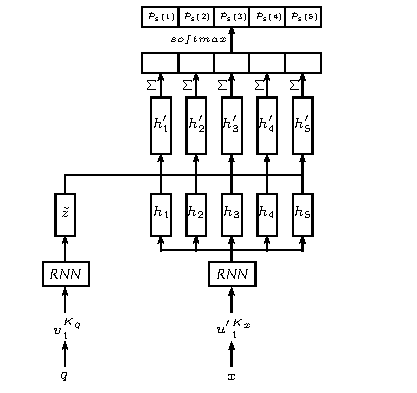
\includegraphics[width=0.9\textwidth]{chapter4/img/fastqa.eps}
  \caption{\small{Uproszczony schemat \textit{FastQA}. Dla czytelności przedstawione jest tylko obliczanie $\hat{P}_s$}. Wektory $u'_i$ to ostateczne reprezentacje słów kontekstu, po dołączeniu zanurzeń znakowych i dwóch dodatkowych cech opisanych poniżej.}
  \label{rysfqa}
\end{figure}

%%%%%%%%%%%%%%%%%%%

\subsubsection{Dodatkowe cechy słów}

Najważniejszą nowością wprowadzaną przez \textit{FastQA} są dwie dodatkowe cechy dla słów kontekstu. Dla każdego $x_i$ są one obliczane na podstawie zależności między $x_i$ a $q$. Okazuje się, że prosta heurystyka mówiąca jak istotne jest dane słowo dla pytania bardzo pomaga podnieść jakość modelu.

Autorzy proponują cechy binarną i ważoną. Binarna stanowi informację o tym, czy słowo znajduje się w pytaniu. Dla $i \in \{1,\dots,K_x\}$:

\[f_b(i, q) =
    \begin{cases}
        1 & \text{jeśli } x_i \text{ występuje w } q \\
        0 & \text{w p.p.} \\[5pt]
    \end{cases}
\]

Przy obliczaniu cechy ważonej najpierw tworzymy macierz podobieństwa pomiędzy słowami kontekstu a słowami pytania. Podobieństwa te są normalizowane funkcją \textit{softmax} i~sumowane po całym $q$.

\[
\begin{aligned}
    \mathrm{sim}_{i,j} &= {\tau_w}^T (u_i \odot v_j) \in \mathbb{R} \\[3pt]
    f_w(i, q) &= \sum\limits_{j \in \{1,\dots,K_q\}} (\mathrm{softmax}(\mathrm{sim}_{\,\cdot,\,j}))_i \\[5pt]
\end{aligned}
\]

\noindent
gdzie $\tau_w \in \mathbb{R}^n$ dla wymiaru zanurzeń $n$. Symbol $^T$ oznacza transpozycję. Parametr $\tau_w$ jest uczony wraz z resztą sieci. Dla każdego $i \in \{1,\dots,K_x\}$ wartości $f_b(i, q)$ i~$f_w(i,q)$ są doklejane do reprezentacji słowa $x_i$ w kroku~1 tworząc zaznaczony na Rysunku~\ref{rysfqa} ciąg ${u'}_1^{K_x}$.

%%%%%%%%%%%%%%%%%%%

\subsubsection{Reprezentacja pytania}

Istotnym elementem modelu jest sposób wyliczania podsumowania pytania, $\tilde{z}$. Wykorzystywany jest do tego tzw. \textit{mechanizm uwagi} (ang. \textit{attention}). Poszczególne wektory ciągu $z_1^{K_q}$ są sumowane z wagami oznaczającymi ich istotność w pytaniu. Odbywa się to podobnie jak w przypadku obliczania $f_w$. Niech $Z = [z_1\ \cdots\ z_{K_q}] \in \mathbb{R}^{m \times K_q}$, gdzie $m$ jest rozmiarem stanu \textit{RNN}:

\[
\begin{aligned}
    \alpha &= \mathrm{softmax}({\tau_q}^T Z) \in \mathbb{R}^{K_q} \\[3pt]
    \tilde{z} &= \sum\limits_{j \in \{1,\dots,K_q\}} \alpha_j z_j \\[5pt]
\end{aligned}
\]

Parametr $\tau_q \in \mathbb{R}^m$ jest uczony. Wykorzystując taką reprezentację $q$ sieć potrafi nauczyć się zwracać uwagę na specyficzne słowa. Na przykład obserwując wiele pytań rozpoczynających się od \textit{when} i mających daty za odpowiedzi, będzie w stanie tak dobrać parametry, żeby słowo \textit{when} dostawało dużą wagę. W praktyce typ pytania mocno ogranicza zakres możliwych odpowiedzi. Mechanizm uwagi pozwala modelowi wykorzystywać ten fakt.

%%%%%%%%%%%%%%%%%%%

\subsubsection{Zanurzenia znakowe}

Zanurzać w przestrzeni wektorowej można nie tylko słowa, ale także pojedyncze znaki. \textit{FastQA} korzysta zarówno z zanurzeń słów jak i z reprezentacji liter. Niech $w$ będzie słowem złożonym ze znaków $c_1,\dots,c_l$, a $m_c$ rozmiarem zanurzeń liter. Możemy zapisać $w$ jako $A = [a_1\ \cdots\ a_l] \in \mathbb{R}^{m_c \times l}$, gdzie $a_i$ jest wektorem dla $c_i$. Macierz $A$ przekształcamy na wektor stałej długości, który będzie reprezentacją $w$ uwzględniającą wzajemne położenie liter w słowie \cite{charemb}.

Wykorzystujemy do tego operację splotu. Dla filtra $H \in \mathbb{R}^{m_c \times k}, k \leq l$ i~opcjonalnego przesunięcia $b \in \mathbb{R}$ definiujemy $A*H \in \mathbb{R}^{l-k+1}$ następująco:
\[(A*H)_i = \tanh(\mathrm{tr}([a_i\ \cdots\ a_{i+k-1}]H^T) + b)\]

Interesującym nas rezultatem jest skalar $\max(A*H)$. Całą operację powtarzamy dla pewnej liczby $n_f$ różnych filtrów, a otrzymane wyniki łączymy w $n_f$-wymiarowy wektor reprezentujący $w$. Wektor ten jest doklejany do zanurzenia $w$ w kroku 1, przed dodaniem cech $f_b$ i $f_w$.

Aby zapewnić dodatkową interakcję pomiędzy dwoma typami zanurzeń słów, autorzy wykorzystują warstwę \textit{highway} \cite{highway}. Niech $\mathbf{w} \in \mathbb{R}^{n+n_f}$ będzie konkatenacją obu reprezentacji $w$. Podlega ona następującym transformacjom:

\[
\begin{aligned}
\mathbf{w}' &= P\mathbf{w}\\
g &= \mathcal{F}_1(\mathbf{w}')\\
\mathbf{w}'' &= \mathcal{F}_2(\mathbf{w}')\\
\tilde{\mathbf{w}} &= g \odot \mathbf{w}' + (1-g) \odot \mathbf{w}'',
\end{aligned}
\]

\noindent
gdzie $P$ jest pewną macierzą, $\mathcal{F}_1$ i $\mathcal{F}_2$ oznaczają warstwy gęste, a $\tilde{\mathbf{w}}$ jest powstałą reprezentacją $w$, do której konkatenowane będą $f_b$ i $f_w$. Warstwa \textit{highway} potrafi nauczyć się proporcji w jakich powinna brać pod uwagę oryginalne i przekształcone wejście.

%%%%%%%%%%%%%%%%%%%

\subsubsection{Pozostałe szczegóły}

W krokach 4. i 5. do kodowania kontekstu dołączamy dodatkowe informacje, które chcemy uwzględnić przy obliczaniu prawdopodobieństw. Najprościej zrobić to przez konkatenację, ale autorzy dołączają dodatkowo iloczyn Hadamarda:

\[
\begin{aligned}[c]
    h'_i &=
    \begin{bmatrix}
        h_i \\
        \tilde{z} \\
        h_i \odot \tilde{z} \\
    \end{bmatrix} \in \mathbb{R}^{3m}
\end{aligned} \ \
\begin{aligned}[c]
    h''_i &=
    \begin{bmatrix}
        h_i \\
        h_{\mathbf{s}} \\
        \tilde{z} \\
        h_i \odot \tilde{z} \\
        h_i \odot h_{\mathbf{s}} \\
    \end{bmatrix} \in \mathbb{R}^{5m}
\end{aligned}
\]


Wektory $h'_i$ oraz $h''_i$ są zwijane do skalarów za pomocą podwójnej warstwy gęstej. Funkcja \textit{softmax} zwraca prawdopodobieństwa:

\[
\begin{aligned}
    &s_i = {\tau_s}^T \mathrm{ReLU}(W_s h'_i + b_s) \in \mathbb{R}\\
    &\hat{P}_s(i \mid q, x) = (\mathrm{softmax}(s))_i \\[10pt]
    &e_i = {\tau_e}^T \mathrm{ReLU}(W_e h''_i + b_e) \in \mathbb{R}\\
    &\hat{P}_e(i \mid \mathbf{s}, q, x) = (\mathrm{softmax}(e))_i\\[5pt]
\end{aligned}
\]

Jako warstwę rekurencyjną, kodującą pytanie i kontekst, wykorzystano dwukierunkowy \textit{LSTM} (\ref{lstm}, \ref{birnn}). Agregację wyników sieci składowych przeprowadzono za pomocą przepuszczenia połączonych stanów przez warstwę gęstą o parametrze $B \in \mathbb{R}^{m \times 2m}$ (bez przesunięcia). Przetwarzanie $q$ i $x$ zostało przeprowadzone za pomocą tych samych parametrów, za wyjątkiem macierzy $B$, która była inna dla pytania i kontekstu. Wartości cech $f_b$~i~$f_w$ dla słów w pytaniu zostały ustalone na 1.

Warstwa zanurzeń podlega procedurze \textit{dropout} \cite{dropout}. Jest to popularna i prosta metodą regularyzacji modelu neuronowego. Każdy element wejścia podlega wyzerowaniu z prawdopodobieństwem $p$, a następnie całość jest mnożona przez $1\, /\, (1-p)$, żeby zachować stałą średnią wyniku. W ten sposób symulujemy uśrednianie wielu modeli. Częstym wyborem $p$ jest $0.5$.

%%%%%%%%%%%%%%%%%%%%%%%%%%%%%%%%%%%%%%%%%%%%%%%%%%%%%%%%%%%%%%%%%%%%%%%%%

\section{Eksperymenty}

Model został wyuczony procedurą \textit{ADAM} (\ref{adam}) na danych \textit{SQuAD}. Wykorzystane zanurzenia słów pochodzą z GloVe i nie były uczone. Zanurzenia znakowe zostały wytrenowane. Co 64\,000 elementów znajdował się punkt kontrolny. Jeśli efektywność na zbiorze testowym malała między punktami kontrolnymi, tempo uczenia było zmniejszane dwukrotnie. Cały proces był dość szybki: 20 przejść po całym zbiorze uczącym zajęło około 4 godziny. Najlepszy rezultat pojawił się już po 9 przejściach.

Miarą jakości modelu jest procent poprawnie udzielonych odpowiedzi na zbiorze testowym. Oficjalny skrypt ewaluacyjny oblicza również miarę F1, stanowiącą balans pomiędzy precyzją (ang. \textit{precision}) i czułością (ang. \textit{recall}). Niestety nie udało mi się zreplikować wyniku z \cite{fastqa}. Model uzyskał 72.34 F1, co jest wynikiem trochę niższym od 76.30 F1 prezentowanym w artykule. Powodem mogą być pojawiające się tam drobne niejasności, które mogłem źle zinterpretować. Nie wykluczam oczywiście błędnej implementacji, chociaż nie potrafiłem znaleźć żadnej usterki. Nie mniej jednak otrzymany wynik jest wystarczająco dobry, żeby przekonać się jak sieć sprawdza się w praktyce.

%%%%%%%%%%%%%%%%%%%

\subsection{Przykłady zastosowania}

Wytrenowana sieć stara się znaleźć podciąg kontekstu, który z największym prawdopodobieństwem jest dobrą odpowiedzią. Sprawdzenie wszystkich możliwych podciągów jest niepraktyczne, więc stosuje się przeszukiwanie wiązkowe (\ref{beamsearch}). Zmniejszenie rozmiaru wiązki do 1 skutkuje jednak dużo szybszym algorytmem zachłannym, który działa tylko nieznacznie gorzej. Takiej właśnie wersji używam.

W tej części zamieszczam przykładowe odpowiedzi udzielone przez model. W~nawiasach znajdują się zwrócone prawdopodobieństwa. Wartości bliskie 1 oznaczają, że sieć jest pewna odpowiedzi. Mniejsze liczby sygnalizują trudniejsze przypadki. Pytania i konteksty pochodzą ze zbioru testowego \textit{SQuAD}. Błędne odpowiedzi są opatrzone dodatkowymi komentarzami.\\\\

%!TEX output_directory = texaux
%!TEX spellcheck
%!TEX root = ../main.tex

\setlength{\abovedisplayskip}{20pt}
\setlength{\belowdisplayskip}{20pt}

\small
\noindent
\textbf{Kontekst}:
\textit{Other green spaces in the city include the Botanic Garden and the University Library Garden. They have extensive botanical collection of rare domestic and foreign plants, while a palm house in the New Orangery displays plants of subtropics from all over the world. Besides, within the city borders, there are also: Pole Mokotowskie (a big park in the northern Mokotów, where was the first horse racetrack and then the airport), Park Ujazdowski (close to the Sejm and John Lennon street), Park of Culture and Rest in Powsin, by the southern city border, Park Skaryszewski by the right Vistula bank, in Praga. The oldest park in Praga, the Praga Park, was established in 1865–1871 and designed by Jan Dobrowolski. In 1927 a Zoological Garden (Ogród Zoologiczny) was established on the park grounds, and in 1952 a bear run, still open today.}

\noindent
\textbf{P}: \textit{What type of space in Warsaw are the Botanic Garden and University Library Garden?}\\
\textbf{O}: \textit{green} (0.81)\\[4pt]
\textbf{P}: \textit{Where is a palm house with subtropic plants from all over the world on display?}\\
\textbf{O}: \textit{New Orangery} (0.35)\\[4pt]
\textbf{P}: \textit{Where was the first horse racetrack located?}\\
\textbf{O}: \textit{pole mokotowskie} (0.34)\\[4pt]
\textbf{P}: \textit{What park is close to John Lennon street?}\\
\textbf{O}: \textit{park ujazdowski} (0.95)\\[4pt]
\textbf{P}: \textit{When was a zoological garden established in the Praga Park?}\\
\textbf{O}: \textit{1865 – 1871} (0.77) (błąd, poprawna odpowiedź: \textit{1927})

\vspace{.3cm}

\noindent
\textbf{Kontekst}:
\textit{Following the cretaceous–paleogene extinction event , the extinction of the dinosaurs and the wetter climate may have allowed the tropical rainforest to spread out across the continent. From 66–34 mya, the rainforest extended as far south as 45\degree. Climate fluctuations during the last 34 million years have allowed savanna regions to expand into the tropics. During the oligocene, for example, the rainforest spanned a relatively narrow band. It expanded again during the middle miocene, then retracted to a mostly inland formation at the last glacial maximum. However, the rainforest still managed to thrive during these glacial periods, allowing for the survival and evolution of a broad diversity of species.}

\noindent
\textbf{P}: \textit{Which type of climate may have allowed the rainforest to spread across the continent?}\\
\textbf{O}: \textit{tropical} (0.52) (błąd, poprawna odpowiedź: \textit{wetter})\\[4pt]
\textbf{P}: \textit{What has allowed for the savanna region to expand into the tropics?}\\
\textbf{O}: \textit{climate fluctuations} (0.98)\\[4pt]
\textbf{P}: \textit{During what time did the rainforest spanned a narrow band?}\\
\textbf{O}: \textit{the oligocene ,} (0.20) (nieścisłość: niepotrzebny przecinek)\\[4pt]
\textbf{P}: \textit{When did it retract to a inland formation?}\\
\textbf{O}: \textit{middle miocene} (0.49)\\[4pt]
\textbf{P}: \textit{Did the rainforest managed to thrive during the glacial periods?}\\
\textbf{O}: \textit{still managed to thrive} (0.31)

\vspace{.3cm}

\noindent
\textbf{Kontekst}:
\textit{QuickBooks sponsored a ``Small Business Big Game'' contest, in which Death Wish Coffee had a 30-second commercial aired free of charge courtesy of QuickBooks. Death Wish Coffee beat out nine other contenders from across the United States for the free advertisement.}

\noindent
\textbf{P}: \textit{What company won a free advertisement due to the QuickBooks contest?}\\
\textbf{O}: \textit{coffee} (0.34) (niepełna odpowiedź, poprawna: \textit{death wish coffee})\\[4pt]
\textbf{P}: \textit{How long was the Death Wish Coffee commercial?}\\
\textbf{O}: \textit{30 - second} (0.78)\\[4pt]
\textbf{P}: \textit{Besides Death Wish Coffee, how many other competitors participated in the contest?}\\
\textbf{O}: \textit{nine} (0.63)\\[4pt]
\textbf{P}: \textit{Which company sponsored a contest called ``Small Business Big Game''?}\\
\textbf{O}: \textit{quickbooks} (1.0)\\[4pt]
\textbf{P}: \textit{How many other contestants did the company, that had their ad shown for free, beat out?}\\
\textbf{O}: \textit{nine} (0.80)

% \vspace{.3cm}

% \noindent
% \textbf{Kontekst}:
% \textit{Despite waiving longtime running back Deangelo Williams and losing top wide receiver Kelvin Benjamin to a torn ACL in the preseason, the Carolina Panthers had their best regular season in franchise history, becoming the seventh team to win at least 15 regular season games since the league expanded to a 16-game schedule in 1978. Carolina started the season 14–0, not only setting franchise records for the best start and the longest single-season winning streak, but also posting the best start to a season by an NFC team in NFL history, breaking the 13–0 record previously shared with the 2009 New Orleans Saints and the 2011 Green Bay Packers. With their NFC-best 15–1 regular season record, the Panthers clinched home-field advantage throughout the NFC playoffs for the first time in franchise history. Ten players were selected to the Pro Bowl (the most in franchise history) along with eight all-pro selections.}

% \noindent
% \textbf{P}: \textit{Who had the best record in the NFC?}\\
% \textbf{O}: \textit{carolina panthers} (0.39)\\[4pt]
% \textbf{P}: \textit{How many Panthers went to the Pro Bowl?}\\
% \textbf{O}: \textit{ten} (0.74)\\[4pt]
% \textbf{P}: \textit{What Panther tore his ACL in the preseason?}\\
% \textbf{O}: \textit{kelvin benjamin} (0.94)\\[4pt]
% \textbf{P}: \textit{What year did the league begin having schedules with 16 games in them?}\\
% \textbf{O}: \textit{1978} (0.99)\\[4pt]
% \textbf{P}: \textit{What year did the the Saints hit a 13-0 record?}\\
% \textbf{O}: \textit{2009} (0.94)

\vspace{.3cm}

\noindent
\textbf{Kontekst}:
\textit{Sir Charles Lyell first published his famous book, Principles of Geology, in 1830. This book, which influenced the thought of Charles Darwin, successfully promoted the doctrine of uniformitarianism. This theory states that slow geological processes have occurred throughout the Earth's history and are still occurring today. In contrast, catastrophism is the theory that Earth's features formed in single, catastrophic events and remained unchanged thereafter. Though Hutton believed in uniformitarianism, the idea was not widely accepted at the time.}

\noindent
\textbf{P}: \textit{First published by Sir Charles Lyell in 1830 this book was called what?}\\
\textbf{O}: \textit{principles of geology} (0.96)\\[4pt]
\textbf{P}: \textit{What doctrine did the doctrine of the Principles of Geology successfully promote?}\\
\textbf{O}: \textit{the doctrine of uniformitarianism} (0.63)\\[4pt]
\textbf{P}: \textit{Which theory states that slow geological processes are still occurring today, and have occurred throughout Earth's history?}\\
\textbf{O}: \textit{uniformitarianism} (0.48)\\[4pt]
\textbf{P}: \textit{Which theory states that Earth's features remained unchanged after forming in one single catastrophic event?}\\
\textbf{O}: \textit{catastrophis}m (1.0)\\[4pt]
\textbf{P}: \textit{Which famous evolutionist was influenced by the book Principles of Geology?}\\
\textbf{O}: \textit{charles darwin} (0.65)

\normalsize

%%%%%%%%%%%%%%%%%%%%%%%%%%%%%%%%%%%%%%%%%%%%%%%%%%%%%%%%%%%%%%%%%%%%%%%%%

\section{Negatywne odpowiedzi} \label{negans}

W zbiorze \textit{SQuAD} każde pytanie jest połączone z pasującym do niego kontekstem i~\textit{FastQA} korzysta z tej własności. Model uczy się znajdować dobre odpowiedzi we fragmentach, które faktycznie je zawierają. W prawdziwym zastosowaniu trudno oczekiwać, że właściwy tekst zawsze będzie pod ręką. Niestety opisana architektura w żaden sposób nie potrafi wykrywać, czy właściwa odpowiedź znajduje się w dostarczonym jej fragmencie. Prawdopodobieństwa, które zwraca, są warunkowe, i nie mogą być rozważane bez kontekstu. Żeby to zaobserwować, weźmy poprzednio przytoczony fragment o bitwie pod Grunwaldem, oraz~krótki tekst o Chopinie:\\

\small
\textbf{1}. \textit{The Battle of Grunwald, First Battle of Tannenberg or Battle of Žalgiris, was fought on \textbf{15 July 1410} during the Polish–Lithuanian–Teutonic War. The alliance of the Kingdom of Poland and the Grand Duchy of Lithuania, led respectively by King Władysław II Jagiełło (Jogaila) and Grand Duke Vytautas, decisively defeated the German–Prussian Teutonic Knights, led by Grand Master Ulrich von Jungingen.\\}

\textbf{2}. \textit{Born on March 1, 1810, in Zelazowa Wola, Poland, Frédéric Chopin, grew up in a middle-class family. He published his first composition at age 7 and began performing one year later. In 1832, he moved to Paris, socialized with high society and was known as an excellent piano teacher. His piano compositions were highly influential.}\footnote{Fragment pochodzi z https://www.biography.com/people/frederic-chopin-9247162}\\

\normalsize
Dla pytania \textit{When was Battle of Grunwald?} algorytm wysoko ocenia odpowiedzi znalezione w obu tekstach:\\

\small
\textbf{O1}: \textit{15 july 1410} (0.95)

\textbf{O2}: \textit{march 1 , 1810} (0.88)\\

\normalsize
Widząc pytanie o czas, model, opierając się na założeniu, że odpowiedź znajduje się w tekście, przypisuje datom duże prawdopodobieństwo. Drugi tekst nie zawiera jednak właściwej odpowiedzi, czego nie jesteśmy w stanie stwierdzić patrząc tylko na wynik.

Ten podrozdział opisuje moją próbę nauczenia \textit{FastQA} wykrywania niepasujących kontekstów. Oczekujemy, że sieć będzie umiała wyłuskać dobrą odpowiedź z~pierwszego z powyższych fragmentów, oraz stwierdzić, że w przypadku drugiego nie potrafi tego zrobić.

Motywacją do przeprowadzenia eksperymentu były problemy napotkane podczas tworzenia chatbota \url{poetwanna.be} (\ref{celpracy}). System miał odpowiadać na pytania dwuetapowo. Najpierw przeprowadzał wyszukiwanie w Wikipedii. Następnie zgromadzone teksty były przetwarzane przez \textit{FastQA}, a najbardziej prawdopodobna odpowiedź stanowiła rezultat algorytmu. Nasza wyszukiwarka była jednak dość prosta, więc nie zawsze udawało się znaleźć pasujące fragmenty. Trudno było ocenić jakość wyniku, ponieważ model mógł zwracać wysokie prawdopodobieństwo odpowiedzi nawet dla niewłaściwych akapitów. Gdyby zamiast tego potrafił je ignorować, współpraca wyszukiwarki i \textit{FastQA} byłaby dużo efektywniejsza.

Pomysł opiera się na lekkiej zmianie procesu uczenia. Oprócz pozytywnych przykładów pokażemy sieci także teksty, które nie zawierają odpowiedzi. Nie ingerujemy w żaden sposób w architekturę \textit{FastQA}, ale dostosowujemy dane do jej ograniczeń. Ponieważ model zakłada, że zawsze musi odpowiedzieć pozytywnie, doklejamy do wszystkich kontekstów sztuczne słowo \textbf{neg}. Uznajemy je za poprawną odpowiedź we wszystkich przypadkach, w których fragment nie odpowiada na pytanie. Fragmenty z przykładu (po tokenizacji, czyli podzieleniu napisu na słowa) będą wyglądały tak:\\

\small
\textit{the battle of grunwald , first battle} [...] \textit{jungingen .} \textbf{neg}

\textit{born on march 1, 1810, in zelazowa} [...] \textit{influential .} \textbf{neg}\\

\normalsize
W pierwszym przypadku nadal spodziewamy się zobaczyć wynik \textit{15 july 1410}. W drugim mamy nadzieję na \textbf{neg}, co pozwoli nam wywnioskować, że fragment nie zawiera właściwej odpowiedzi. Podczas uczenia dalej korzystamy z ustalonych zanurzeń GloVe, za wyjątkiem wektora dla słowa \textbf{neg}, który jest optymalizowany.

\subsection{Wzbogacanie danych}

Przygotowałem cztery dodatkowe zestawy danych uczących. Dwa z nich są przerobionymi wersjami \textit{SQuAD}:

\begin{itemize}
    \item \texttt{SQuAD-rng} to zbiór uczący \textit{SQuAD} z pomieszanymi kontekstami. Każde pytanie dostało losowo wybrany, niezawierający odpowiedzi, i niepasujący do niego tematycznie fragment.

    \item \texttt{SQuAD-cut} zawiera te same pary $(q, x)$, co dane uczące \textit{SQuAD}, ale w każdej parze z $x$ wycięte zostało zdanie zawierające odpowiedź. Sprawia to, że teksty są na temat, ale nie zawierają odpowiedzi. Obserwacja tego zbioru może pomóc sieci zrozumieć, że nawet mocno związany tematycznie fragment nie musi być właściwy.
\end{itemize}

Robot \texttt{poetwanna.be} szukał odpowiedzi w Wikipedii, co starałem się wziąć pod uwagę w procesie uczenia. W pozostałych dwóch zbiorach pytania pochodzą ze \textit{SQuAD}u, a konteksty z Wikipedii. Akapity w danych \textit{SQuAD} mogą mieć inną charakterystykę niż te zwracane przez wyszukiwarkę. Ich powiązanie z pytaniem również może wyglądać inaczej. Jeśli więc wszystkie przykłady z Wikipedii byłyby negatywne, model mógłby nauczyć się odrzucać je ze względu na cechy inne niż brak właściwej odpowiedzi. Mając to na uwadze, jeden z poniższych zbiorów zawiera pozytywne konteksty:

\begin{itemize}
    \item \texttt{Wiki-pos} składa się z pytań \textit{SQuAD} połączonych z pozytywnymi akapitami znalezionymi w Wikipedii. Nie udało się znaleźć pasujących fragmentów dla każdego pytania, więc ten zbiór zawiera tylko 52\,600 elementów, co stanowi $61\%$ całego \textit{SQuAD}.
    \item \texttt{Wiki-neg} jest zbudowany tak jak \texttt{Wiki-pos}, ale zawiera tylko negatywne przykłady. Akapity pochodzą z wyników wyszukiwarki, więc są w pewien sposób tematycznie związane z pytaniami.
\end{itemize}

Analogiczne zbiory zostały utworzone dla zbioru testowego \textit{SQuAD}, \texttt{SQuAD-dev}. Korzystałem z \texttt{SQuAD-rng-dev}, \texttt{Wiki-pos-dev}, \texttt{Wiki-neg-dev}, oraz \texttt{SQuAD-dev}, żeby zmierzyć efektywność sieci wyuczonych w różnych warunkach.

\subsection{Wyniki}

Eksperyment polegał na wzbogacaniu oryginalnego zbioru uczącego \textit{SQuAD} różnymi kombinacjami czterech dodatkowych zestawów danych. Weryfikacja jakości modelu polegała na sprawdzeniu ile kontekstów zostało odrzuconych z~każdego ze~zbiorów testowych. Idealny model udzieliłby poprawnych odpowiedzi dla każdego przykładu w \texttt{Wiki-pos-dev} i oryginalnym \texttt{SQuAD-dev}, a odrzucił wszystkie fragmenty znajdujące się w \texttt{SQuAD-rng-dev} i \texttt{Wiki-neg-dev}.

Wyniki przedstawione są w Tabeli~\ref{squadtab}. Każdy wiersz reprezentuje jeden model. Kolumna \textbf{Dane} zawiera zbiory danych, o które został rozszerzony zbiór uczący \textit{SQuAD}. Sprawdzam również jak bardzo postawienie przed architekturą dodatkowej trudności wpływa na wynik w oryginalnym zadaniu. \textbf{Pos F1} oznacza F1 na \texttt{SQuAD-dev}, gdy model nie może udzielić odpowiedzi negatywnej (bez doklejania \textbf{neg}). \textbf{Neg F1} jest mierzone tak samo, ale ze słowem \textbf{neg}. Wartości te stanowią miarę pogorszenia jakości rozwiązywania podstawowego problemu \textit{SQuAD}.

W Tabeli~\ref{squadtab} widzimy, że wybór danych uczących ma olbrzymi wpływ na wynik. Lepiej przygotowane negatywne przykłady prawdopodobnie poprawiłyby rezultat. Można też zauważyć kompromis między liczbą odrzucanych niewłaściwych kontekstów a liczbą pozytywnych przykładów, które rozwiązujemy poprawnie. Wybór ``najlepszego'' modelu jest z tego powodu trudny.

Ostatecznie bot \texttt{poetwanna.be} nie korzystał z negatywnych modeli; tracimy zbyt dużo poprawnych odpowiedzi, żeby sobie na to pozwolić. Doświadczenie pokazuje jednak, że odrzucanie złych kontekstów ma potencjał. Odpowiednie modyfikacje sieci lub danych uczących mogłyby umożliwić zastosowanie tego pomysłu w praktyce.

\setlength{\tabcolsep}{3pt}
\begin{table}[ht]
    \centering
    \caption{Procent odrzuconych fragmentów dla różnych modeli}
    \label{squadtab}
    \begin{tabular}{|l|r|r|r|r|r|r|}
        \hline
        \rowcolor[gray]{.85}
        \textbf{Dane} & \textbf{Wiki-pos} & \textbf{SQuAD} & \textbf{Wiki-neg} & \textbf{SQuAD-rng} & \textbf{neg F1} & \textbf{pos F1}\\
        \hline
         & 0 & 0 & 0.01 & 0.03 & 72.36 & 72.34\\
        \hline
        \makecell[l]{\texttt{SQuAD-rng}} & 0.01 & 0.02 & 0.07 & 0.98 & 69.73 & 70.34\\
        \hline
        \makecell[l]{\texttt{SQuAD-cut}} & 0.25 & 0.22 & 0.62 & 1 & 60.99 & 70.5\\
        \hline
        \makecell[l]{\texttt{Wiki-neg}} & 0.53 & 0.27 & 0.92 & 0.53 & 55.11 & 70.6\\
        \hline
        \makecell[l]{\texttt{Wiki-neg}\\\texttt{Wiki-pos}} & 0.4 & 0.23 & 0.87 & 0.65 & 58.72 & 70.19\\
        \hline
        \makecell[l]{\texttt{SQuAD-rng}\\\texttt{Wiki-neg}\\\texttt{Wiki-pos}} & 0.35 & 0.23 & 0.82 & 0.99 & 57.83 & 69.15\\
        \hline
        \makecell[l]{\texttt{SQuAD-rng}\\\texttt{SQuAD-cut}} & 0.26 & 0.22 & 0.63 & 1 & 61.05 & 71.05\\
        \hline
    \end{tabular}\par
\end{table}

\subsection{Przykłady negatywnych odpowiedzi}

Ta część zawiera przykłady odpowiedzi udzielanych przez przedostatni model z~Tabeli~\ref{squadtab}. Najpierw przypomnijmy wcześniej przytoczone fragmenty o bitwie pod Grunwaldem i Chopinie. \textbf{p} oznacza model pozytywny, a \textbf{n} negatywny.\\

\small
\textbf{1}. \textit{The Battle of Grunwald, First Battle of Tannenberg or Battle of Žalgiris, was fought on \textbf{15 July 1410} during the Polish–Lithuanian–Teutonic War. The alliance of the Kingdom of Poland and the Grand Duchy of Lithuania, led respectively by King Władysław II Jagiełło (Jogaila) and Grand Duke Vytautas, decisively defeated the German–Prussian Teutonic Knights, led by Grand Master Ulrich von Jungingen.\\}

\textbf{2}. \textit{Born on March 1, 1810, in Zelazowa Wola, Poland, Frédéric Chopin, grew up in a middle-class family. He published his first composition at age 7 and began performing one year later. In 1832, he moved to Paris, socialized with high society and was known as an excellent piano teacher. His piano compositions were highly influential.}\\

\textbf{O1 p}: \textit{15 july 1410} (0.95)\\\indent
\textbf{O1 n}: \textit{15 july 1410} (0.54)

\textbf{O2 p}: \textit{march 1 , 1810} (0.88)\\\indent
\textbf{O2 n}: \textbf{neg} (0.96)\\

\normalsize
Model negatywny zachował się zgodnie z oczekiwaniami. Potrafił znaleźć właściwą odpowiedź w pierwszym tekście oraz stwierdzić, że drugi jej nie zawiera. Należy jednak zwrócić uwagę na mniejsze prawdopodobieństwo w pierwszym przypadku. Oznacza to dużo większą niepewność modelu.

Dalej zamieszczam kilka kolejnych przykładów. Na temat każdego akapitu zadaję trzy pytania z możliwością odpowiedzi, i trzy, na które nie da się odpowiedzieć na podstawie fragmentu. Pytania, które są w pewien sposób związane z tekstem, są znacznie trudniejsze. Brak komentarza oznacza poprawną odpowiedź. Podobnie jak powyżej, można zaobserwować większą niepewność modelu negatywnego na pytaniach pozytywnych.\\\\

%!TEX output_directory = texaux
%!TEX spellcheck
%!TEX root = ../main.tex

\setlength{\abovedisplayskip}{20pt}
\setlength{\belowdisplayskip}{20pt}

\small
\noindent
\textbf{Kontekst}:
\textit{Jacksonville is the largest city by population in the U.S. state of Florida, and the largest city by area in the contiguous United States. It is the county seat of Duval County, with which the city government consolidated in 1968. Consolidation gave Jacksonville its great size and placed most of its metropolitan population within the city limits; with an estimated population of 853,382 in 2014, it is the most populous city proper in Florida and the southeast, and the 12th most populous in the United States . Jacksonville is the principal city in the Jacksonville metropolitan area, with a population of 1,345,596 in 2010. }

\noindent
\textbf{P}: \textit{Which Florida city has the biggest population?}\\
\textbf{O p}: \textit{jacksonville} (0.92)\\
\textbf{O n}: \textit{jacksonville} (0.55)\\[5pt]
\textbf{P}: \textit{What was the population Jacksonville city as of 2010?}\\
\textbf{O p}: \textit{1 , 345 , 596} (1.0)\\
\textbf{O n}: \textit{1 , 345 , 596} (0.41)\\[5pt]
\textbf{P}: \textit{Based on population alone, what is Jacksonville's ranking in the United States?}\\
\textbf{O p}: \textit{12th} (0.63)\\
\textbf{O n}: \textit{12th} (0.45)\\[10pt]
\textbf{P}: \textit{What is the population of Los Angeles?}\\
\textbf{O p}: \textit{853 , 382} (0.68) (błąd, brak odpowiedzi)\\
\textbf{O n}: \textbf{neg} (0.63)\\[5pt]
\textbf{P}: \textit{What is the smallest city in Oklahoma?}\\
\textbf{O p}: \textit{jacksonville} (0.80) (błąd, brak odpowiedzi)\\
\textbf{O n}: \textbf{neg} (0.60)\\[5pt]
\textbf{P}: \textit{Who founded Jacksonville?}\\
\textbf{O p}: \textit{population} (0.22) (błąd, brak odpowiedzi)\\
\textbf{O n}: \textit{population in the u . s . state of florida} (0.35) (błąd, brak odpowiedzi)

\vspace{.3cm}

\noindent
\textbf{Kontekst}:
\textit{Luther justified his opposition to the rebels on three grounds. First, in choosing violence over lawful submission to the secular government, they were ignoring Christ's counsel to ``Render unto Caesar the things that are Caesar's''; St. Paul had written in his epistle to the Romans 13:1–7 that all authorities are appointed by God and therefore should not be resisted. This reference from the Bible forms the foundation for the doctrine known as the divine right of kings, or, in the German case, the divine right of the princes. Second, the violent actions of rebelling, robbing, and plundering placed the peasants ``outside the law of God and Empire'', so they deserved ``death in body and soul, if only as highwaymen and murderers.'' Lastly, Luther charged the rebels with blasphemy for calling themselves ``Christian brethren'' and committing their sinful acts under the banner of the Gospel.}

\noindent
\textbf{P}: \textit{What were the protesters doing with Christ's counsel?}\\
\textbf{O p}: \textit{render unto caesar the things} (0.41) (błąd, poprawna odpowiedź: \textit{ignoring})\\
\textbf{O n}: \textbf{neg} (0.36) (błąd, poprawna odpowiedź: \textit{ignoring})\\[5pt]
\textbf{P}: \textit{By whom did St Paul say all authorities were appointed?}\\
\textbf{O p}: \textit{god} (1.0)\\
\textbf{O n}: \textit{god} (0.89)\\[5pt]
\textbf{P}: \textit{What is this doctrine of God appointing authorities called?}\\
\textbf{O p}: \textit{the divine right of kings} (0.64)\\
\textbf{O n}: \textbf{neg} (0.39) (błąd, odrzucenie dobrego fragmentu)\\[10pt]
\textbf{P}: \textit{Who was Martin Luther?}\\
\textbf{O p}: \textit{the rebels with blasphemy} (0.29) (błąd, brak odpowiedzi)\\
\textbf{O n}: \textbf{neg} (0.72)\\[5pt]
\textbf{P}: \textit{How many epistles did St. Paul write?}\\
\textbf{O p}: \textit{13 : 1 – 7} (0.62) (błąd, brak odpowiedzi)\\
\textbf{O n}: \textit{three} (0.41) (błąd, brak odpowiedzi)\\[5pt]
\textbf{P}: \textit{When did Luther annouce his three treatises?}\\
\textbf{O p}: \textit{second} (0.22) (błąd, brak odpowiedzi)\\
\textbf{O n}: \textbf{neg} (0.96)

\vspace{.3cm}

\noindent
\textbf{Kontekst}:
\textit{In a report, published in early February 2007 by the Ear Institute at the University College London, and Widex, a Danish hearing aid manufacturer, Newcastle was named as the noisiest city in the whole of the UK, with an average level of 80.4 decibels. The report claimed that these noise levels would have a negative long-term impact on the health of the city's residents. The report was criticized, however, for attaching too much weight to readings at arbitrarily selected locations, which in Newcastle's case included a motorway underpass without pedestrian access.}

\noindent
\textbf{P}: \textit{What's the average decibel level of noise in Newcastle?}\\
\textbf{O p}: \textit{80 . 4 decibels} (0.72)\\
\textbf{O n}: \textit{80 . 4 decibels} (0.83)\\[5pt]
\textbf{P}: \textit{What type of impact can the residents of Newcastle expect the city's noise to have on them?}\\
\textbf{O p}: \textit{negative long - term} (0.35)\\
\textbf{O n}: \textit{negative long - term impact} (0.41)\\[5pt]
\textbf{P}: \textit{What was one location the noise readings in Newcastle were taken at?}\\
\textbf{O p}: \textit{motorway underpass} (0.25)\\
\textbf{O n}: \textbf{neg} (0.27) (błąd, odrzucenie dobrego fragmentu)\\[10pt]
\textbf{P}: \textit{When was Widex founded?}\\
\textbf{O p}: \textit{february 2007} (0.82) (błąd, brak odpowiedzi)\\
\textbf{O n}: \textbf{neg} (0.35)\\[5pt]
\textbf{P}: \textit{How many UK citizens have hearing problems?}\\
\textbf{O p}: \textit{80 . 4} (0.46) (błąd, brak odpowiedzi)\\
\textbf{O n}: \textbf{neg} (0.57)\\[5pt]
\textbf{P}: \textit{What is the average length of a motorway?}\\
\textbf{O p}: \textit{80 . 4 decibels} (0.93) (błąd, brak odpowiedzi)\\
\textbf{O n}: \textit{80 . 4 decibels} (0.61) (błąd, brak odpowiedzi)

% \vspace{.3cm}

% \noindent
% \textbf{Kontekst}:
% \textit{}

% \noindent
% \textbf{P}: \textit{}\\
% \textbf{O p}: \textit{} ()\\
% \textbf{O n}: \textit{} ()\\[5pt]
% \textbf{P}: \textit{}\\
% \textbf{O p}: \textit{} ()\\
% \textbf{O n}: \textit{} ()\\[5pt]
% \textbf{P}: \textit{}\\
% \textbf{O p}: \textit{} ()\\
% \textbf{O n}: \textit{} ()\\[10pt]
% \textbf{P}: \textit{}\\
% \textbf{O p}: \textit{} ()\\
% \textbf{O n}: \textit{} ()\\[5pt]
% \textbf{P}: \textit{}\\
% \textbf{O p}: \textit{} ()\\
% \textbf{O n}: \textit{} ()\\[5pt]
% \textbf{P}: \textit{}\\
% \textbf{O p}: \textit{} ()\\
% \textbf{O n}: \textit{} ()\\

\normalsize

%!TEX output_directory = texaux
%!TEX spellcheck
%!TEX root = ../main.tex

\setlength{\abovedisplayskip}{20pt}
\setlength{\belowdisplayskip}{20pt}

\chapter{Podsumowanie}

Sieci neuronowe znalazły w ostatnich latach szerokie zastosowanie w dziedzinie przetwarzania języka, na czym naturalnie skorzystały systemy dialogowe. Generowanie zdań słowo po słowie jest ciekawą perspektywą, która uwalnia nas od konieczności ręcznej konstrukcji wypowiedzi i daje maszynie możliwość wykazania oryginalności. Niestety obecnie to rozwiązanie boryka się z dość fundamentalnymi przeszkodami. Różnorodność wypowiedzi i dobre zrozumienie kontekstu są bardzo trudne do uzyskania. Automatyczna ocena jakości generowanych dialogów dobrze korelująca z osądem ludzkim cały czas pozostaje otwartym problemem. Niemniej jednak jest to interesująca gałąź sztucznej inteligencji, ciesząca się zainteresowaniem w środowiskach naukowych.

Wyszukiwanie odpowiedzi na pytania w zadanym kontekście daje znacznie bardziej imponujące wyniki. Najlepsze systemy osiągają w tym zadaniu skuteczność bardzo bliską ludzkiej, co pozwala z powodzeniem wykorzystywać je w praktyce. Sporą trudnością pozostaje jednak znalezienie odpowiedniego tekstu do konkretnego pytania. Wykorzystanie standardowych technik przeszukiwania nie zawsze daje pożądane rezultaty. Optymalny system powinien być wyposażony w wyszukiwarkę specjalnie dostosowaną do tego problemu lub potrafić samemu ocenić dopasowanie otrzymywanych fragmentów.

Niemałą rolę w rozwoju systemów dialogowych odgrywa rywalizacja. Konkursy takie jak The Alexa Prize\footnote{\url{https://developer.amazon.com/alexaprize}}, Nagroda Loebnera, czy NIPS Conversational Intelligence Challenge stanowią coroczną motywację dla naukowców i programistów. Łatwa dostępność chatbotów, na przykład za pośrednictwem Facebooka, sprawia, że są one coraz mocniej obecne w świadomości publicznej. Mnogość interaktywnych aplikacji asystujących użytkownikowi pokazuje, że roboty konwersacyjne mają również potencjał w biznesie. Systemy dialogowe stają się więc coraz bardziej popularne i~zaawansowane.

\clearpage
\clearpage

\addcontentsline{toc}{chapter}{Bibliografia}
\bibliography{bibliography}
\bibliographystyle{apalike}

\end{document}
